\documentclass[11pt,a4paper]{article}
\usepackage[margin=2.2cm]{geometry}
\usepackage[T1]{fontenc}
\usepackage[utf8]{inputenc}
\usepackage{lmodern}
\usepackage{microtype}
\usepackage{graphicx}
\usepackage{booktabs}
\usepackage{tabularx}
\usepackage{array}
\usepackage{multirow}
\usepackage{amsmath,amssymb}
\usepackage{enumitem}
\usepackage{caption}
\usepackage{subcaption}
\usepackage{float}
\usepackage{longtable}
\usepackage{listings}
\usepackage{xcolor}
\usepackage{hyperref}
\usepackage{tikz}
\usetikzlibrary{arrows.meta,positioning,shapes.geometric,fit}

\hypersetup{
    colorlinks=true,
    linkcolor=black,
    citecolor=black,
    urlcolor=blue,
    pdftitle={Progress Report: Input-Aware Inference on NVIDIA Jetson Orin Nano},
    pdfauthor={Eren Olmez}
}
\setlist[itemize]{leftmargin=1.4em,itemsep=0.25em,topsep=0.35em}
\setlist[enumerate]{leftmargin=1.6em,itemsep=0.25em,topsep=0.35em}
\captionsetup{font=small,labelfont=bf}
\renewcommand{\arraystretch}{1.12}
\setlength{\parindent}{0pt}
\setlength{\parskip}{0.45em}
\newcommand{\code}[1]{\texttt{#1}}
\newcommand{\pp}{~pp}
\newcommand{\mJ}{~mJ}
\newcommand{\ms}{~ms}
\newcommand{\W}{~W}
\newcommand{\img}{~image}

\lstset{
  basicstyle=\ttfamily\small,
  columns=fullflexible,
  frame=single,
  breaklines=true,
  showstringspaces=false
}

\title{\textbf{Progress Report: Input-Aware Inference\\on NVIDIA Jetson Orin Nano}}
\author{Eren Olmez\\M.Sc. Thesis Progress Report}
\date{1 October 2026}

\begin{document}
\maketitle
\vspace{-1.2em}



\section{Progress summary}

This report documents the development of an input-aware inference system for CIFAR-100 on the NVIDIA Jetson Orin Nano. The work combines structured pruning, TensorRT deployment, hardware power measurements, and lightweight routers that choose an inference model before classification. The current repository contains the PC training pipeline, Jetson benchmarks, structural ResNet-34/50 pruning checks, and the data used in the reported figures.

The main result is a negative but useful systems finding. Candidate-only measurements suggested that routing could reduce energy and latency. End-to-end measurements show that these gains often disappear after feature extraction, routing, transfers, and synchronization are included. Under a strict 0.5 percentage-point accuracy allowance, a static p10 model is currently better than every tested dynamic policy: depending on batch size, it saves 8.80--10.13\% energy and 7.16--7.98\% latency relative to p0. Dynamic routing becomes competitive only under looser accuracy limits, and its clearest advantage is a small energy improvement at a 1.5-point allowance for batches 64 and 128.

The cover date is retained from the original report. This revision includes measurements completed through 3 October 2026.

\section{Research question}

The thesis asks whether an input-only router can select among pre-trained deployment configurations and reduce measured Jetson energy or latency without exceeding a specified accuracy loss. The Jetson Orin Nano is the primary platform. Static pruning, quantization, and TensorRT optimization establish the candidate configurations; dynamic routing is evaluated only after these static alternatives have been measured directly.

The literature review led to three related directions:

\begin{enumerate}
    \item \textbf{Dynamic model/configuration selection.} A lightweight router inspects the input and selects among candidate models or compressed configurations. This is closest to IF-CNN and PERTINENCE, and is also related to routing among computation levels in CARN \cite{shu2018ifcnn,shende2026pertinence,gaire2025carn}.
    \item \textbf{Early-exit networks.} Intermediate classifiers terminate easy samples before the full network is executed. BranchyNet and MSDNet are canonical examples; Predictive Exit and later work address the overhead and hardware implications of exit decisions \cite{branchynet,msdnet,predictiveexit}.
    \item \textbf{Hardware-aware multi-objective optimization.} Model choice, pruning, precision, power mode, GPU frequency, latency, throughput, and energy can be treated as a joint configuration problem rather than optimized independently. PolyThrottle, E4, and hardware-algorithm co-optimization studies are representative of this direction \cite{polythrottle,e4,zniber2026}.
\end{enumerate}

The current implementation focuses mainly on the first and third directions. Early exit remains a useful baseline for later comparison. The present router is \emph{input-only}: it selects a TensorRT configuration before any candidate classifier is executed.

\subsection{Definition of input difficulty}

A key conclusion from the literature review is that ``difficulty'' should not be treated as a fixed visual property of an image. Blur, entropy, texture, or edge density may correlate with difficulty, but they do not directly measure whether a particular model will classify the sample correctly. A more operational definition is:

\begin{quote}
An input is difficult when additional computation is required to satisfy the task constraint.
\end{quote}

This connects several apparently different methods. Early-exit systems estimate whether deeper computation is needed from confidence or entropy; DynamicDet defines difficulty through the improvement offered by a stronger detector; PERTINENCE constructs an offline oracle based on which model can solve a sample at acceptable cost \cite{dynamicdet,shende2026pertinence}. In the present work, candidate-model predictions are generated offline and the router is trained to infer a suitable computation level from the input alone.

\section{Methodological revisions}

Three changes are important when comparing early and current results. First, router fitting, calibration, and evaluation now use disjoint class-stratified subsets of the CIFAR-100 test set (6,000/2,000/2,000 images). This removed candidate-training images from router supervision. Second, p0 is the reporting baseline. The offline cheapest-correct oracle is used only to construct or study supervision and is not presented as a deployable accuracy result. Third, energy and latency are optimized separately and every Jetson claim includes the complete decision and inference path.

The early study compared 22 routers on the PC. Later Jetson experiments showed that candidate-only cost estimates were insufficient because routing overhead was comparable with the saving obtained from mildly pruned models. The implementation therefore moved from per-image decisions to one decision per batch, added intermediate p10/p20 candidates, exported TinyCNN to TensorRT, and measured static and dynamic alternatives under the same accuracy allowances.

\section{Experimental platform and implemented pipeline}

The repository is organized by execution environment. PC-side experiments train and compare routers; Jetson-side experiments build TensorRT engines, measure hardware behavior, and benchmark complete routed systems. The implementation currently contains four main components:

\begin{itemize}
    \item \code{architecture\_tests/resnet\_pruning}: structural validation of Torch-Pruning on ResNet-34 and ResNet-50;
    \item \code{pc\_tests/router\_benchmark}: input-only router training, calibration, repeated evaluation, and candidate-cost modeling;
    \item \code{jetson\_tests}: ONNX/TensorRT export, FP32/FP16/INT8 evaluation, power-mode sweeps, and end-to-end dynamic-routing benchmarks;
    \item \code{tests}: unit tests covering feature extraction, deterministic data splitting, TinyCNN output shape, and routing-policy behavior.
\end{itemize}

At the time of this report, all 20 repository unit tests pass in the supplied environment.

\subsection{Dataset, candidate models, and data split}

The active routing experiment uses CIFAR-100. The candidate pool consists of a distilled ResNet-18 family with structured pruning levels
\[
\mathcal{M}=\{p0,p10,p20,\ldots,p90\},
\]
where \code{p0} is the unpruned FP32 baseline and \code{p10}--\code{p90} denote increasing requested pruning ratios. For router development, the CIFAR-100 test set is deterministically divided into 6,000 fit images, 2,000 calibration images, and 2,000 evaluation images, stratified by class. Learner seeds 42--51 are used for repeated comparisons.

The router receives only the current input image at runtime. Candidate networks are used offline to construct supervision and cost tables; they are not executed before the router makes its runtime choice. This distinction is important: the current approach is pre-inference model selection rather than a sequential cascade.

\subsection{Cost objectives and calibration}

Energy and latency are treated as separate objectives. Candidate energy is constructed from measured power and latency,
\begin{equation}
E_m = P_m\,t_m,
\label{eq:candidate-energy}
\end{equation}
with the units chosen so that power in watts multiplied by milliseconds gives millijoules per image. The routing policy is calibrated on a disjoint calibration set to minimize selected-candidate cost while allowing at most a one-percentage-point reduction relative to the unpruned \code{p0} baseline.

For correctness-style routers, the implemented utility has the form
\begin{equation}
U_m(x)=\hat{q}_m(x)-\lambda\frac{C_m}{C_{p0}},
\label{eq:utility}
\end{equation}
where $\hat{q}_m(x)$ estimates candidate correctness or advantage, $C_m$ is measured candidate cost, and $\lambda$ is selected on calibration data. The fallback is always \code{p0} when no cheaper feasible policy is found. This makes the baseline explicit and avoids assuming that pruning ratio or model index is a monotonic proxy for accuracy or cost.

\begin{figure}[H]
\centering
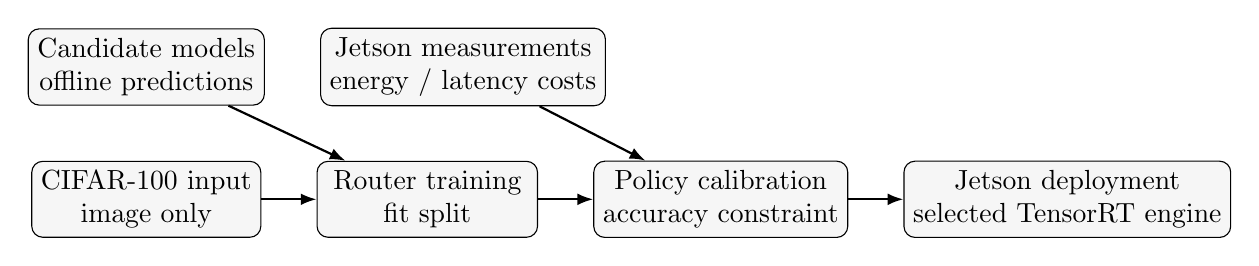
\begin{tikzpicture}[
    node distance=7mm and 7mm,
    box/.style={draw,rounded corners,align=center,minimum height=9mm,minimum width=28mm,fill=gray!7},
    arr/.style={-{Latex[length=2mm]},thick}
]
\node[box] (offline) {Candidate models\\offline predictions};
\node[box,right=of offline] (costs) {Jetson measurements\\energy / latency costs};
\node[box,below=of offline] (input) {CIFAR-100 input\\image only};
\node[box,right=of input] (router) {Router training\\fit split};
\node[box,right=of router] (cal) {Policy calibration\\accuracy constraint};
\node[box,right=of cal] (deploy) {Jetson deployment\\selected TensorRT engine};
\draw[arr] (offline) -- (router);
\draw[arr] (costs) -- (cal);
\draw[arr] (input) -- (router);
\draw[arr] (router) -- (cal);
\draw[arr] (cal) -- (deploy);
\end{tikzpicture}
\caption{Implemented workflow. Candidate networks provide offline supervision; runtime routing uses only the input image. The final Jetson benchmark measures the complete path rather than candidate cost alone.}
\label{fig:pipeline}
\end{figure}

\section{Static optimization work: pruning and quantization}

\subsection{ResNet-18 pruning/precision deployment}

The current Jetson benchmark reproduces the earlier ResNet-18 pruning and precision sweep with additional power, energy, and temperature measurements. The most stable accuracy trend is that pruning causes the dominant accuracy loss while FP16 has almost no accuracy penalty and calibrated INT8 causes only a small additional drop for this model family. For example, the unpruned model obtains 73.70\% top-1 accuracy in FP32/FP16 and 73.28\% in INT8, while the 30\% pruned models obtain 71.51\%, 71.48\%, and 71.27\%, respectively.

\begin{figure}[H]
\centering
\begin{subfigure}[t]{0.49\textwidth}
    \centering
    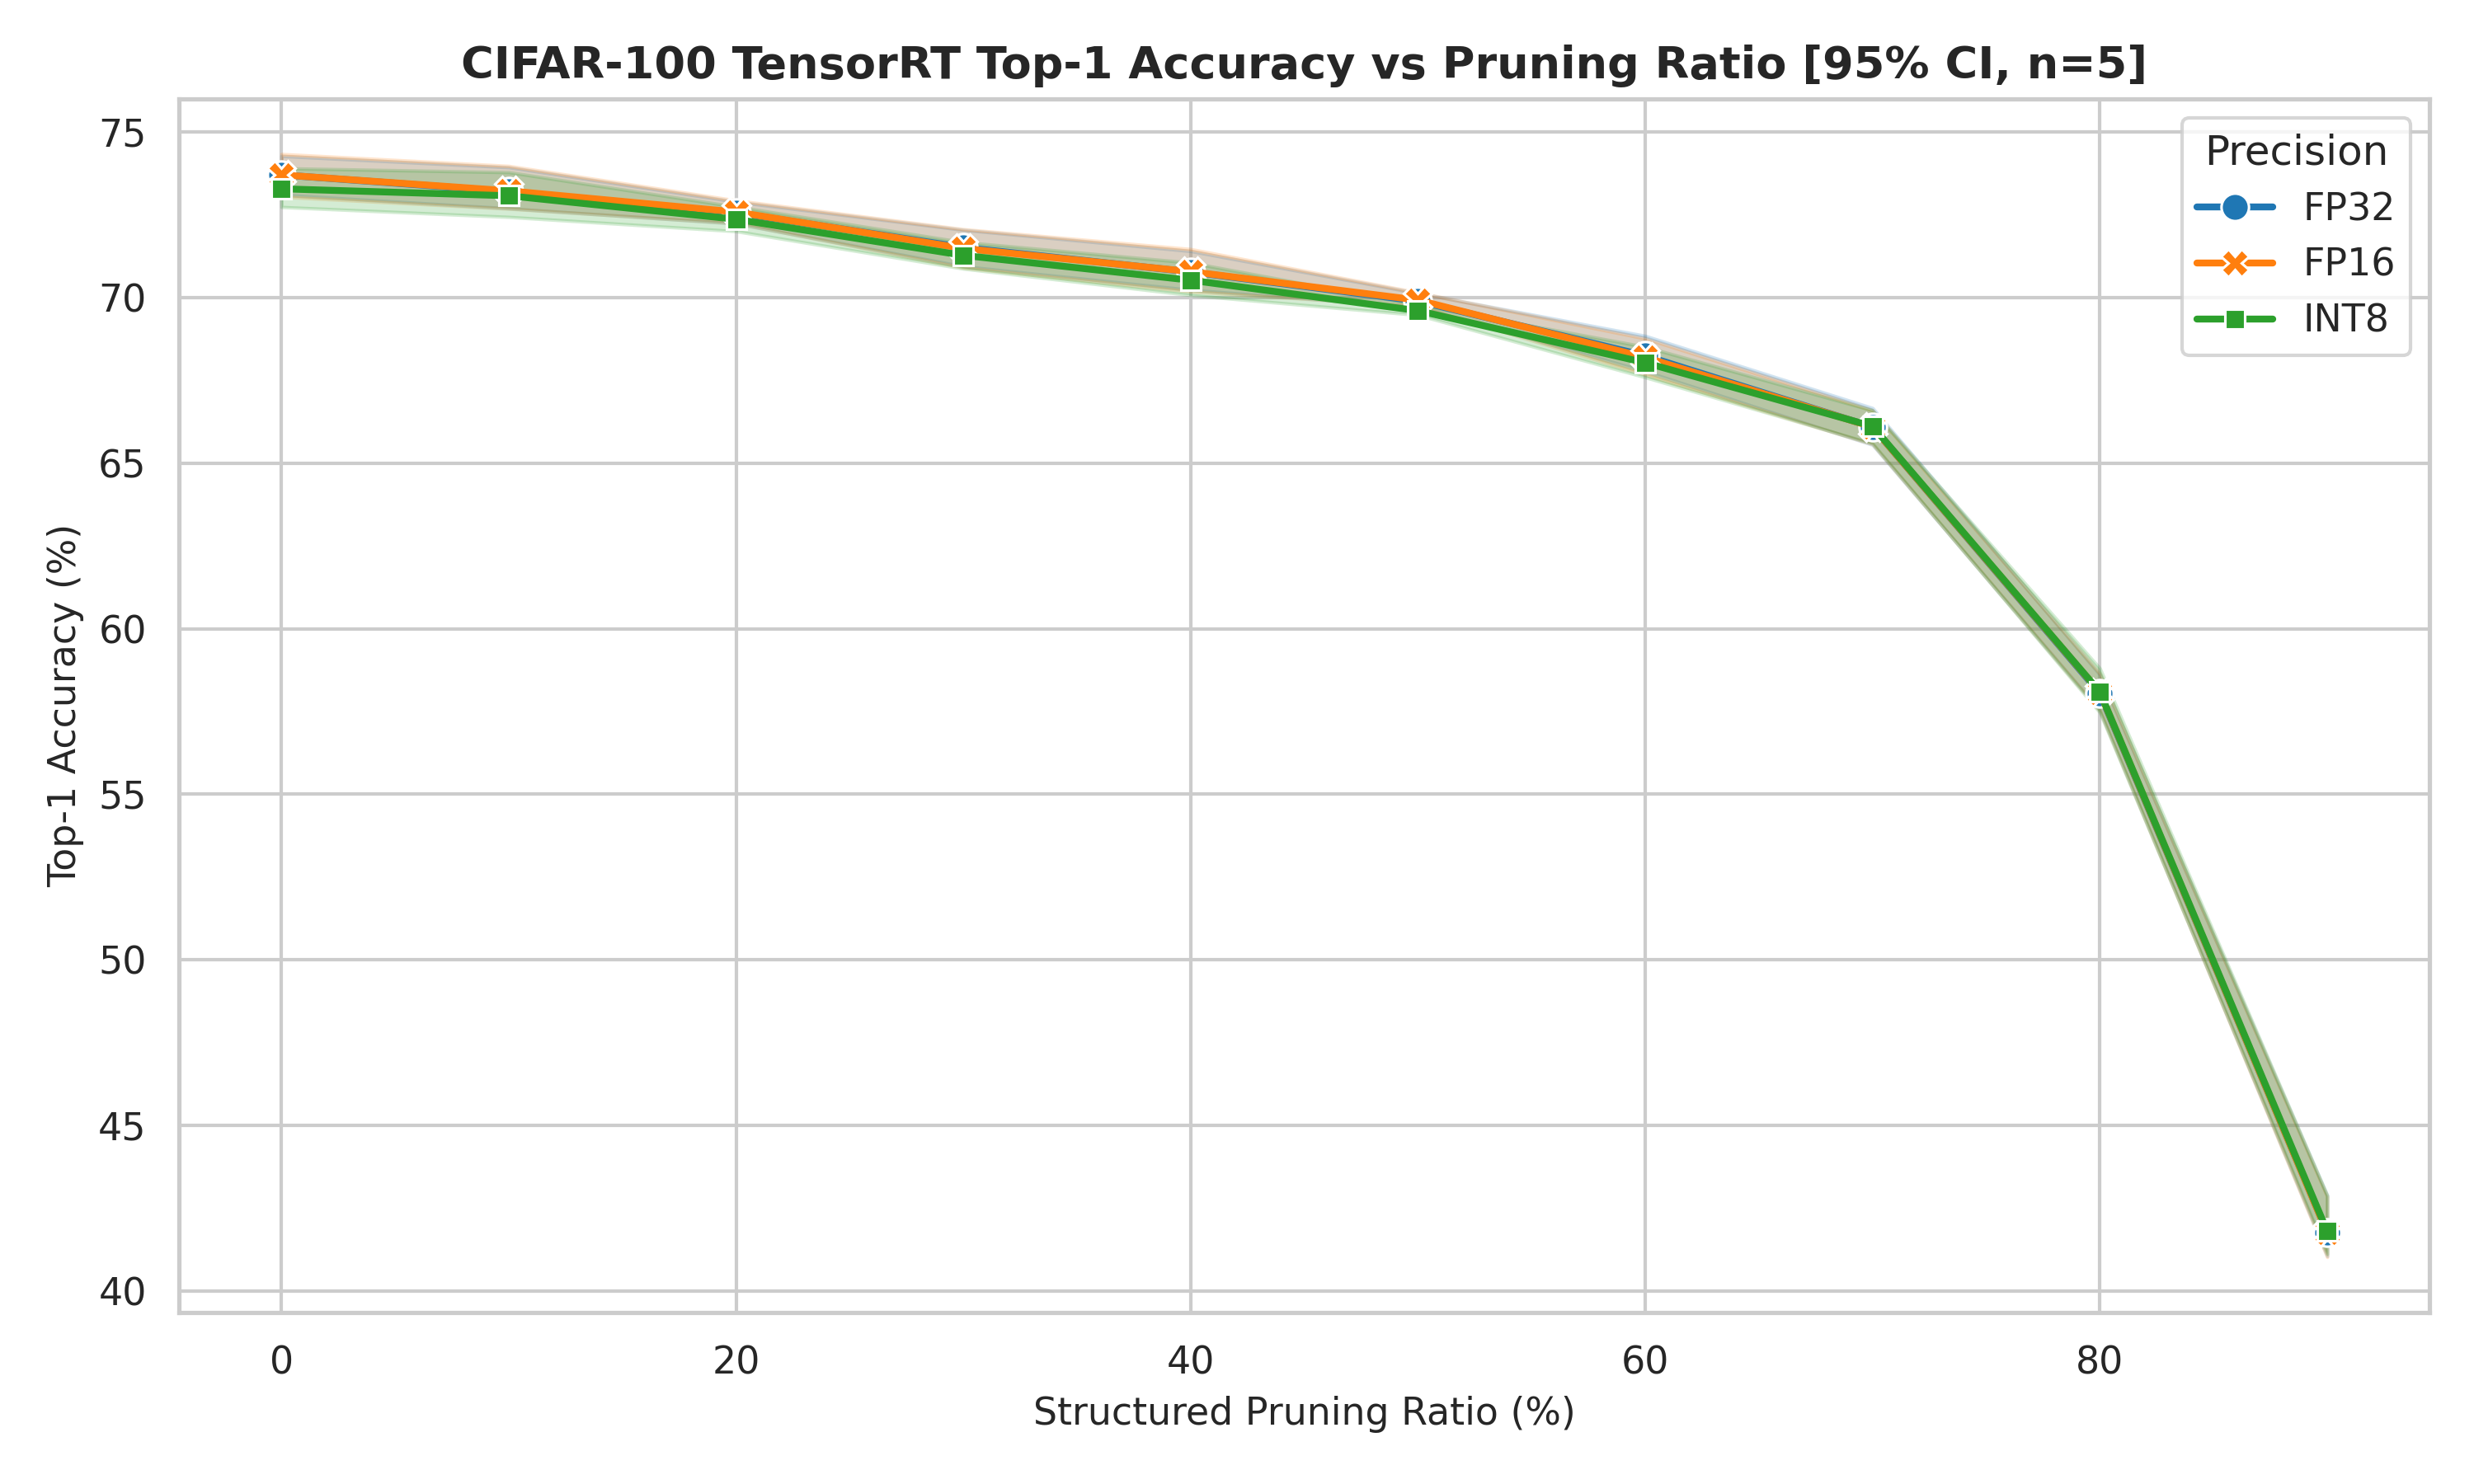
\includegraphics[width=\linewidth]{assets/accuracy_trt.png}
    \caption{Top-1 accuracy versus requested pruning ratio.}
\end{subfigure}\hfill
\begin{subfigure}[t]{0.49\textwidth}
    \centering
    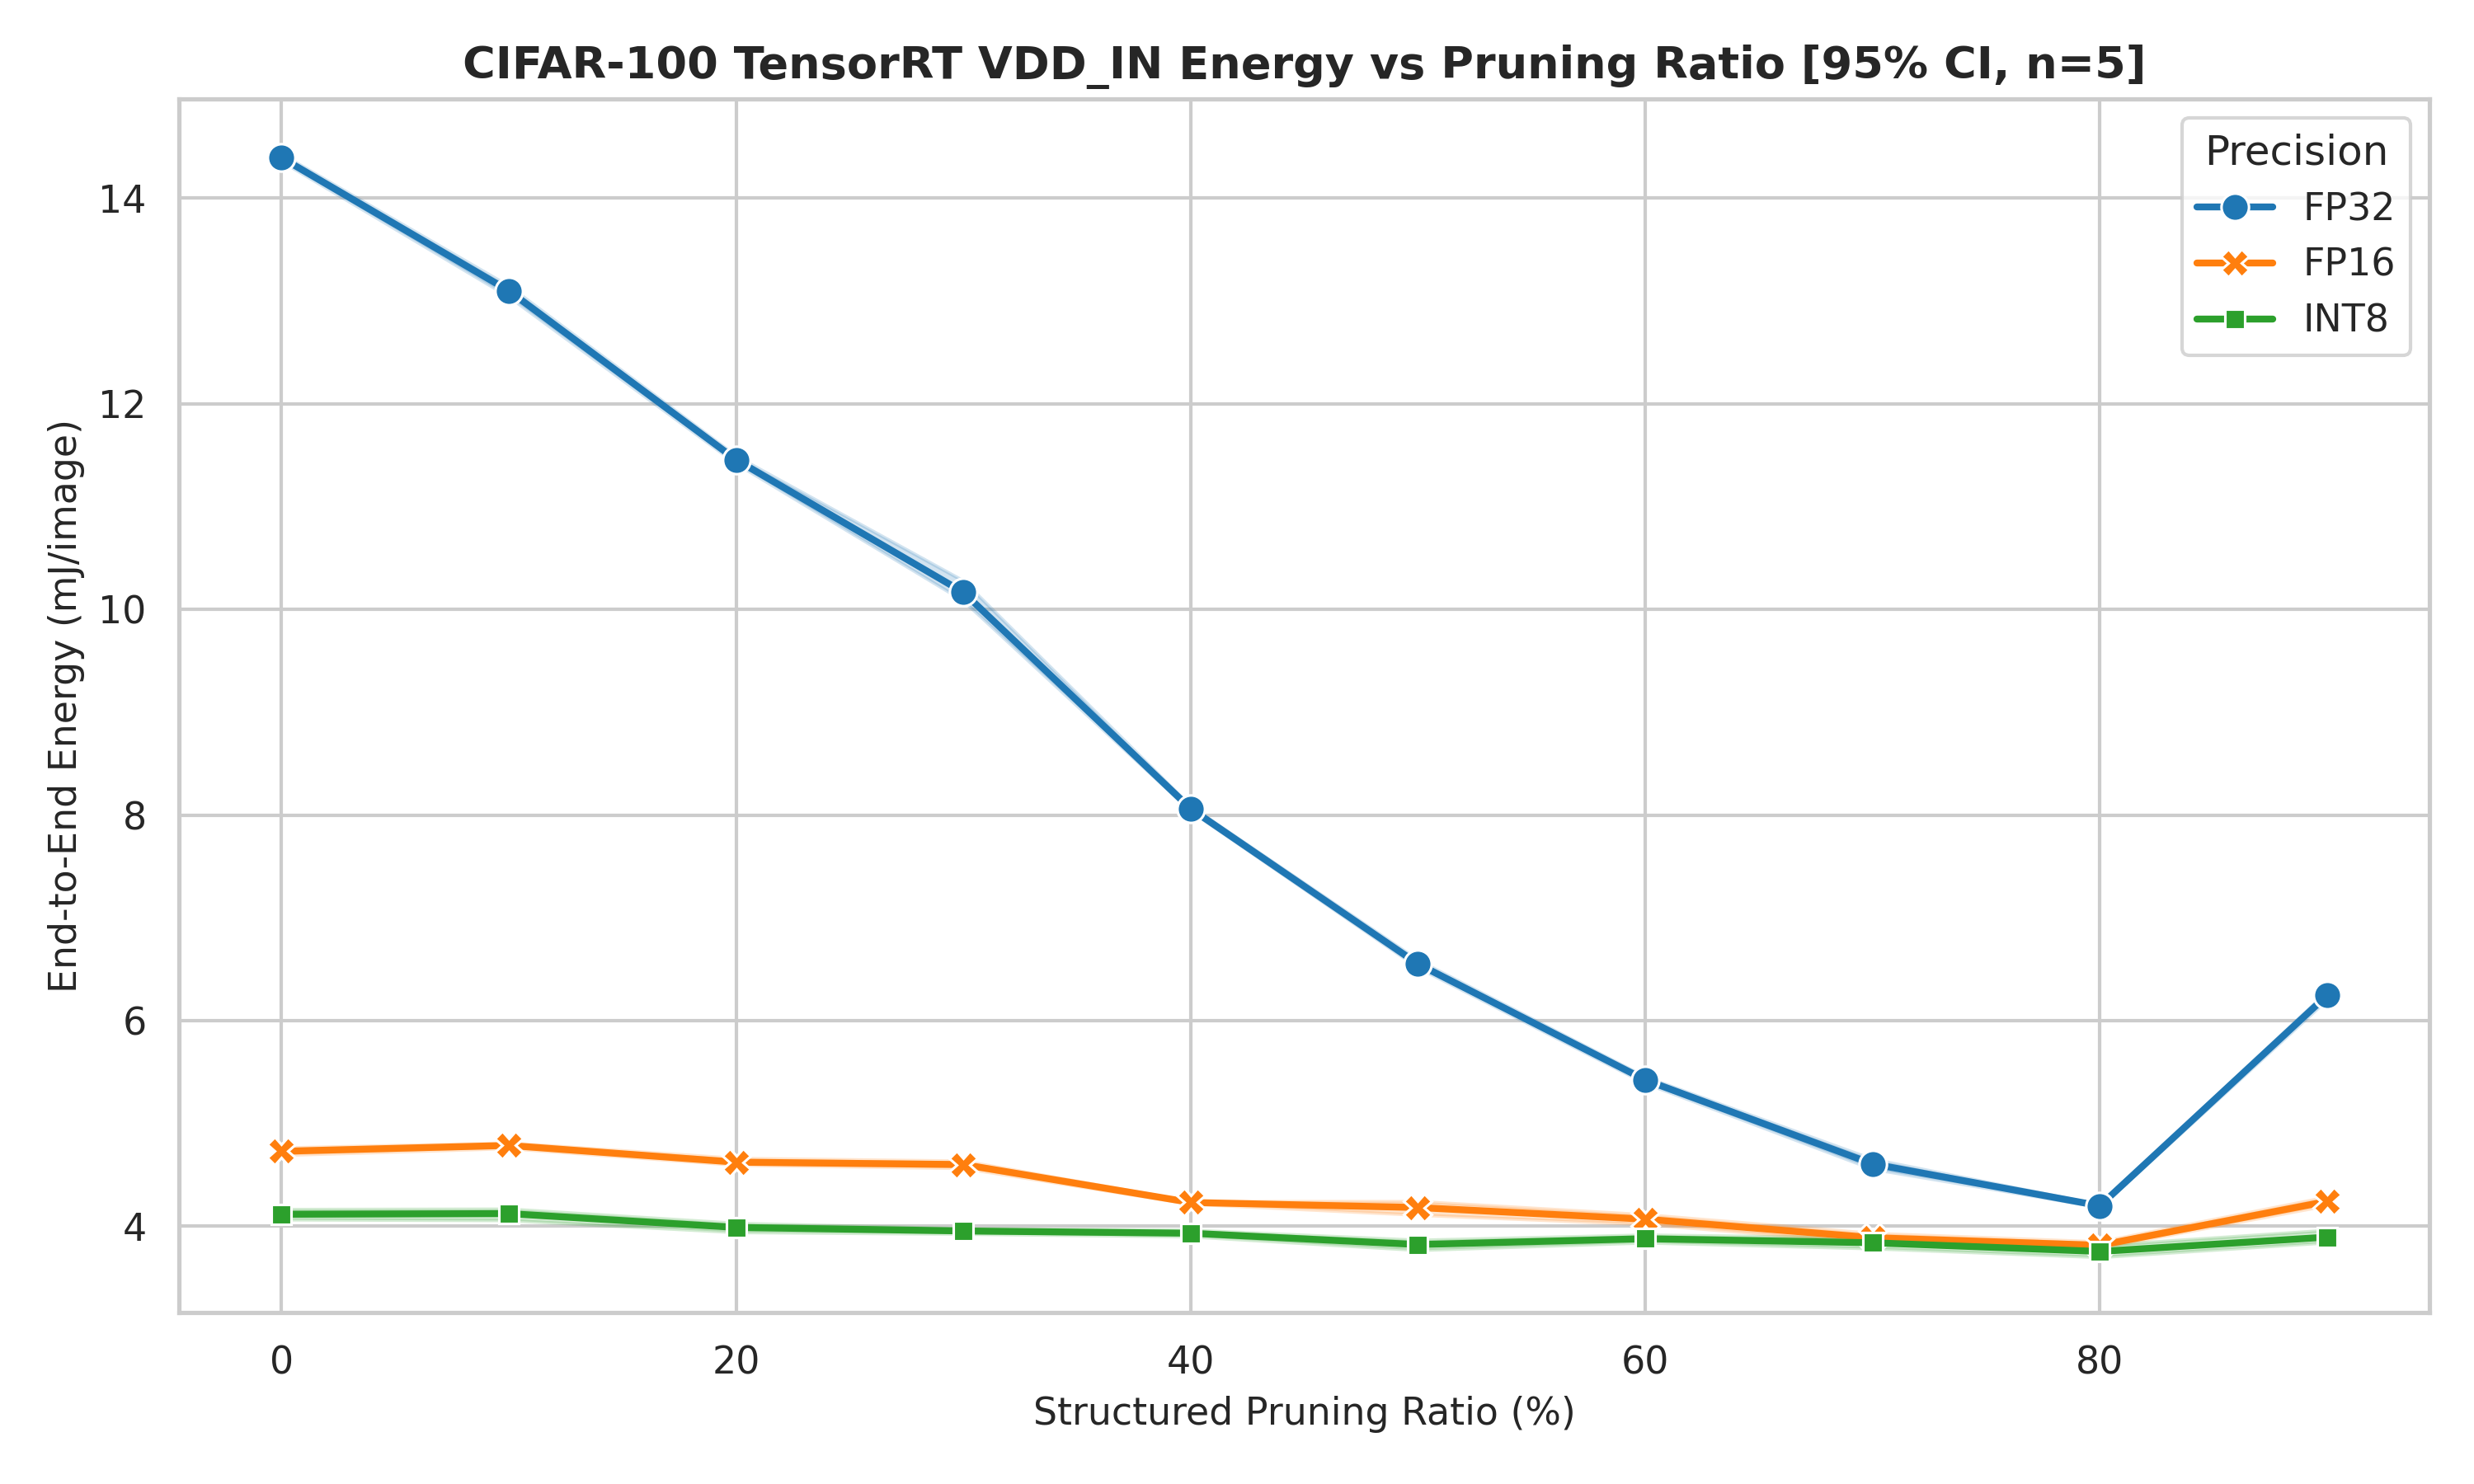
\includegraphics[width=\linewidth]{assets/energy_e2e_trt.png}
    \caption{Measured end-to-end VDD\_IN energy.}
\end{subfigure}
\caption{TensorRT pruning/precision sweep on the Jetson. The figures show why pruning ratio alone is not a sufficient deployment metric: accuracy, precision support, latency, and measured energy must be considered jointly.}
\label{fig:pruning-precision}
\end{figure}

The TensorRT results also show non-monotonic deployment behavior. In FP32, pruning substantially reduces energy until high pruning levels, but the 90\% configuration becomes worse than the 80\% configuration in both latency/throughput behavior and energy. FP16 and INT8 are already fast enough that pruning often changes engine size more clearly than end-to-end latency. This supports using measured hardware cost rather than assuming that fewer parameters or MACs imply proportionally lower latency or energy.

\subsection{ResNet-34/50 Torch-Pruning compatibility}

A separate structural experiment was added to verify that the intended pruning method can be applied to larger ResNet architectures before investing in full training and fine-tuning. Randomly initialized CIFAR-100 ResNet-34 and ResNet-50 models were pruned with dependency-aware channel pruning from 10\% to 90\%. All 18 architecture/ratio combinations produced valid 100-class outputs.

The experiment also exposed an important high-pruning anomaly: at 90\% requested pruning, parameter reduction continues to increase, but the reported MAC reduction becomes worse than at 80\%. For ResNet-34 the 90\% setting reduces parameters by 98.03\% but MACs by only 77.06\%, compared with a 96.55\% MAC reduction at 80\%. ResNet-50 shows the same qualitative behavior. This validates the pruning mechanism structurally but also confirms that extreme requested ratios cannot be interpreted naively. A full ResNet-34/50 accuracy study still requires trained baselines and equal-schedule fine-tuning.

\section{Input-only router benchmark on the PC}

The PC router benchmark compares different input representations under the same images, candidate pool, cost table, data split, and accuracy constraint. Its purpose is to measure how well each router predicts a useful computation level before Jetson deployment.

\subsection{Router families}

The current benchmark contains 22 methods. They can be grouped into four practical families:

\begin{itemize}
    \item \textbf{Handcrafted features + classical ML.} Basic, enhanced, compact, and texture descriptors are fed to XGBoost, Extra Trees, Random Forest, Ridge, or k-NN. The compact descriptor has 46 features; the texture descriptor has 450 features and adds color histograms, HOG, and LBP to global/spatial statistics.
    \item \textbf{Frozen learned embedding.} A frozen ImageNet MobileNetV3-Small produces an embedding that is then used by XGBoost. This gives richer semantic information but has much higher router cost.
    \item \textbf{Direct-image TinyCNN.} A small depthwise-separable CNN receives 8$\times$8, 16$\times$16, or 32$\times$32 normalized images and predicts either a scalar difficulty target or per-candidate correctness.
    \item \textbf{Thumbnail MLP.} An 8$\times$8 image is flattened and classified by a small MLP, providing a simple learned baseline.
\end{itemize}

Three target constructions are compared. \emph{Scalar} targets encode the cost-ordered cheapest-correct candidate. \emph{Correctness} targets estimate the probability that each candidate is correct. \emph{Advantage} targets estimate each candidate's correctness difference relative to \code{p0}. The latter two are combined with the calibrated utility in Eq.~\eqref{eq:utility}.

\subsection{PC-side results}

The PC benchmark measures selected-candidate cost and router overhead separately. Candidate energy/latency does not yet include the router itself, so these numbers are intentionally treated as screening results rather than final deployment claims.

\begin{table}[H]
\centering
\small
\caption{Representative 10-seed PC router results. ``Saving'' refers to selected candidate cost only; router overhead is measured separately on the PC. All listed methods satisfy the one-percentage-point evaluation budget in all 10 seeds.}
\begin{tabularx}{\textwidth}{@{}lXrrrr@{}}
\toprule
Objective & Router & Accuracy & $\Delta$ vs p0 & Candidate saving & Router overhead \\
\midrule
Energy & Frozen MobileNet + XGB scalar & 72.17\% & -0.57\pp & 14.24\% & 17.28\ms \\
Energy & Texture XGB balanced & 72.06\% & -0.69\pp & 7.76\% & 2.92\ms \\
Energy & Compact XGB shallow & 72.41\% & -0.35\pp & 7.02\% & 2.30\ms \\
Energy & TinyCNN-32 scalar & 72.32\% & -0.43\pp & 6.98\% & 2.11\ms \\
\addlinespace
Latency & TinyCNN-8 scalar & 72.39\% & -0.36\pp & 7.29\% & 1.95\ms \\
Latency & Compact XGB shallow & 72.19\% & -0.56\pp & 7.20\% & 2.20\ms \\
Latency & TinyCNN-32 correctness & 72.28\% & -0.47\pp & 7.16\% & 2.10\ms \\
\bottomrule
\end{tabularx}
\label{tab:pc-router}
\end{table}

Two observations are already useful. First, richer semantic information can improve model selection: the frozen MobileNet embedding obtains the largest stable candidate-energy saving. However, its 17\ms PC routing cost is too high for the intended deployment. Second, cheap routers are competitive: compact handcrafted XGBoost and TinyCNN variants produce roughly 7\% candidate savings while remaining close to baseline accuracy. This justified moving both router types to the Jetson rather than selecting a winner solely from PC results.

\section{Jetson hardware characterization}

The Jetson Orin Nano 8 GB used in the experiment exposes native 7 W and 15 W \code{nvpmodel} modes. The repository records supported fixed GPU clocks of 306, 408, 510, 612, and 624.75 MHz, with the available subset depending on the power mode. The power profile label is treated as a board configuration, not as an exact instantaneous GPU power cap. Actual module power is measured from \code{VDD\_IN} through \code{tegrastats}; the combined CPU/GPU/CV rail is recorded separately.

One representative FP16 unpruned ResNet-18 model was swept across the supported operating points at batch sizes 1 and 32. The result is a clear example of why average watts are not enough: the lower-power setting can consume more energy per image because the inference takes longer.

\begin{table}[H]
\centering
\small
\caption{Selected hardware-sweep results for the unpruned FP16 ResNet-18.}
\begin{tabular}{@{}lrrrrr@{}}
\toprule
Operating point & Batch & E2E latency & VDD\_IN & Energy/image & Accuracy \\
\midrule
15 W / 306 MHz & 1 & 4.673 ms & 7.262 W & 33.930 mJ & 73.75\% \\
7 W / 306 MHz & 1 & 5.300 ms & 6.543 W & 34.685 mJ & 73.65\% \\
7 W / 408 MHz & 1 & 4.401 ms & 6.766 W & 29.785 mJ & 73.69\% \\
15 W / 612 MHz & 1 & \textbf{2.857 ms} & 8.961 W & 25.597 mJ & 73.75\% \\
15 W / 624.75 MHz & 1 & 2.875 ms & 8.616 W & \textbf{24.765 mJ} & 73.70\% \\
\addlinespace
15 W / 408 MHz & 32 & 0.574 ms & 9.142 W & \textbf{5.257 mJ} & 73.75\% \\
15 W / 612 MHz & 32 & \textbf{0.553 ms} & 9.771 W & 5.399 mJ & 73.75\% \\
\bottomrule
\end{tabular}
\label{tab:power-sweep}
\end{table}

\begin{figure}[H]
\centering
\begin{subfigure}[t]{0.49\textwidth}
    \centering
    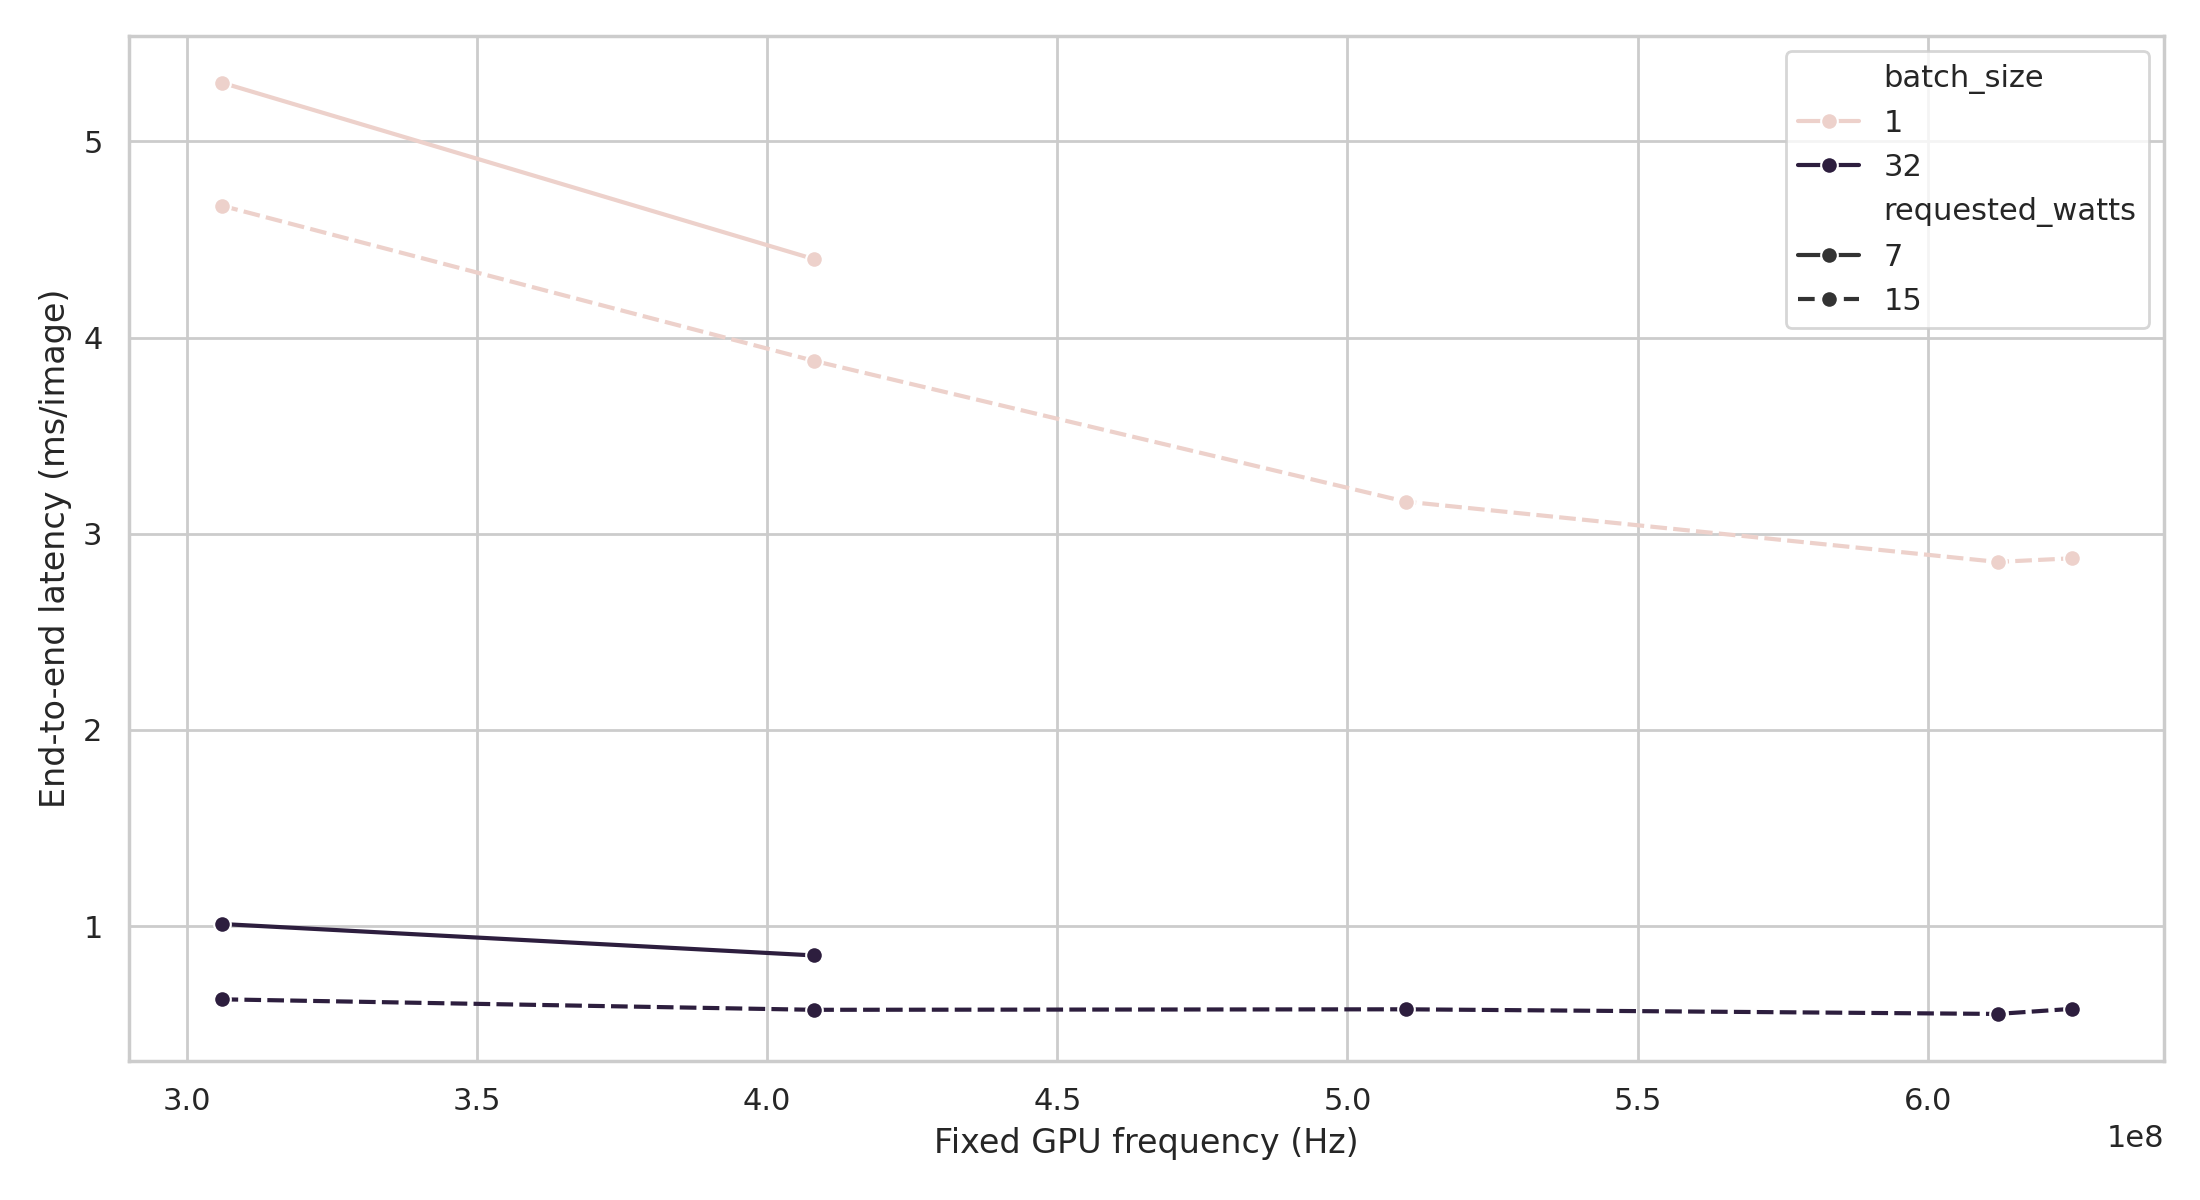
\includegraphics[width=\linewidth]{assets/latency_by_power.png}
    \caption{End-to-end latency across GPU clocks.}
\end{subfigure}\hfill
\begin{subfigure}[t]{0.49\textwidth}
    \centering
    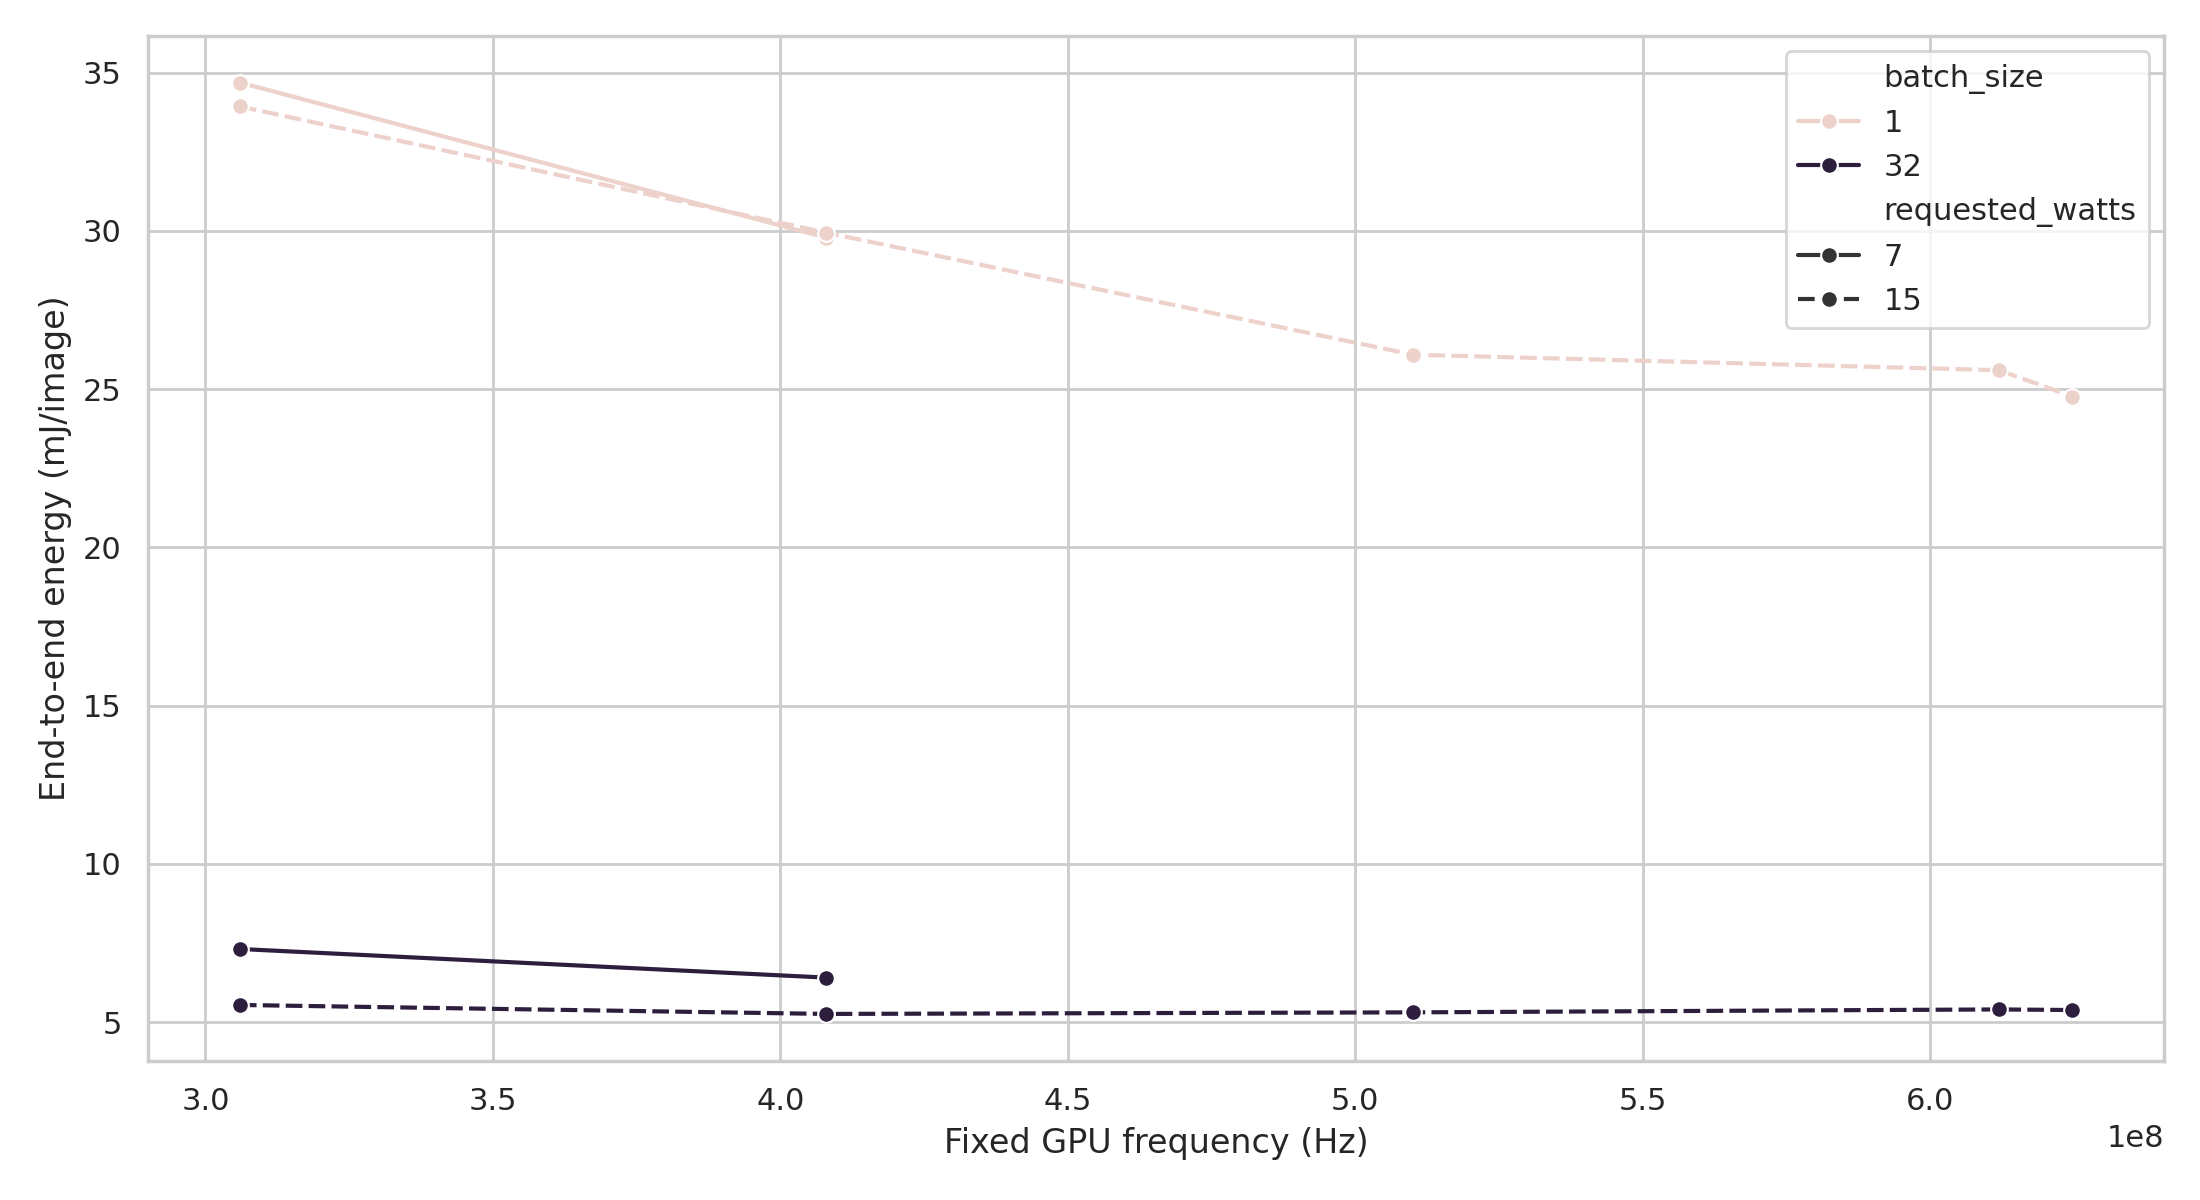
\includegraphics[width=\linewidth]{assets/energy_by_power.png}
    \caption{End-to-end energy across GPU clocks.}
\end{subfigure}
\caption{Hardware characterization. The energy-optimal clock is workload- and batch-dependent; the lowest-watt mode is not necessarily the lowest-energy mode.}
\label{fig:hardware-sweep}
\end{figure}

For batch 1, 612 MHz minimizes latency while 624.75 MHz minimizes measured energy. At batch 32, 612 MHz is again the fastest point, but 408 MHz has the lowest measured energy. This supports a hardware-aware optimization formulation in which GPU frequency/power mode is a decision variable rather than a fixed experimental constant.

\section{End-to-end dynamic routing on the Jetson}

The most important implementation step was moving from model-only estimates to a complete Jetson benchmark. The dynamic benchmark evaluates the same fixed 2,000 CIFAR-100 images for every system, repeats each full system three times, and includes input analysis, router inference, routing decision, preprocessing, selected TensorRT engine execution, synchronization, and integrated power. This is the relevant measurement for deciding whether routing is actually useful.

Two separate experiments were run:
\begin{itemize}
    \item an \textbf{energy-calibrated} policy at 15 W / 624.75 MHz;
    \item a \textbf{latency-calibrated} policy at 15 W / 612 MHz.
\end{itemize}

\begin{table}[H]
\centering
\small
\caption{Best representative full-system routed results versus the unpruned FP32 baseline. Negative saving means the routed system is worse.}
\begin{tabularx}{\textwidth}{@{}lXrrrrr@{}}
\toprule
Objective & System & Accuracy & Latency & Energy & Router overhead & Saving vs p0 \\
\midrule
Energy & p0 baseline & 72.75\% & 10.442 ms & 85.999 mJ & 0.043 ms & --- \\
Energy & Compact XGB s48 & 72.50\% & 12.958 ms & 95.616 mJ & 2.635 ms & -11.18\% energy \\
\addlinespace
Latency & p0 baseline & 72.75\% & 10.569 ms & 86.326 mJ & 0.044 ms & --- \\
Latency & TinyCNN-8 s45 & 72.20\% & 12.389 ms & 91.241 mJ & 2.697 ms & -17.23\% latency \\
\bottomrule
\end{tabularx}
\label{tab:jetson-routing}
\end{table}

The best energy router selected \code{p0} for 511 images, \code{p10} for 1,338, and \code{p20} for 151. The fastest latency router selected \code{p0} for 394 images, \code{p10} for 971, \code{p20} for 574, \code{p50} for 59, and \code{p60} for two. The policy is therefore not exploiting a large enough cost gap to compensate for approximately 2.6--2.7 ms of routing overhead per image.

\begin{figure}[H]
\centering
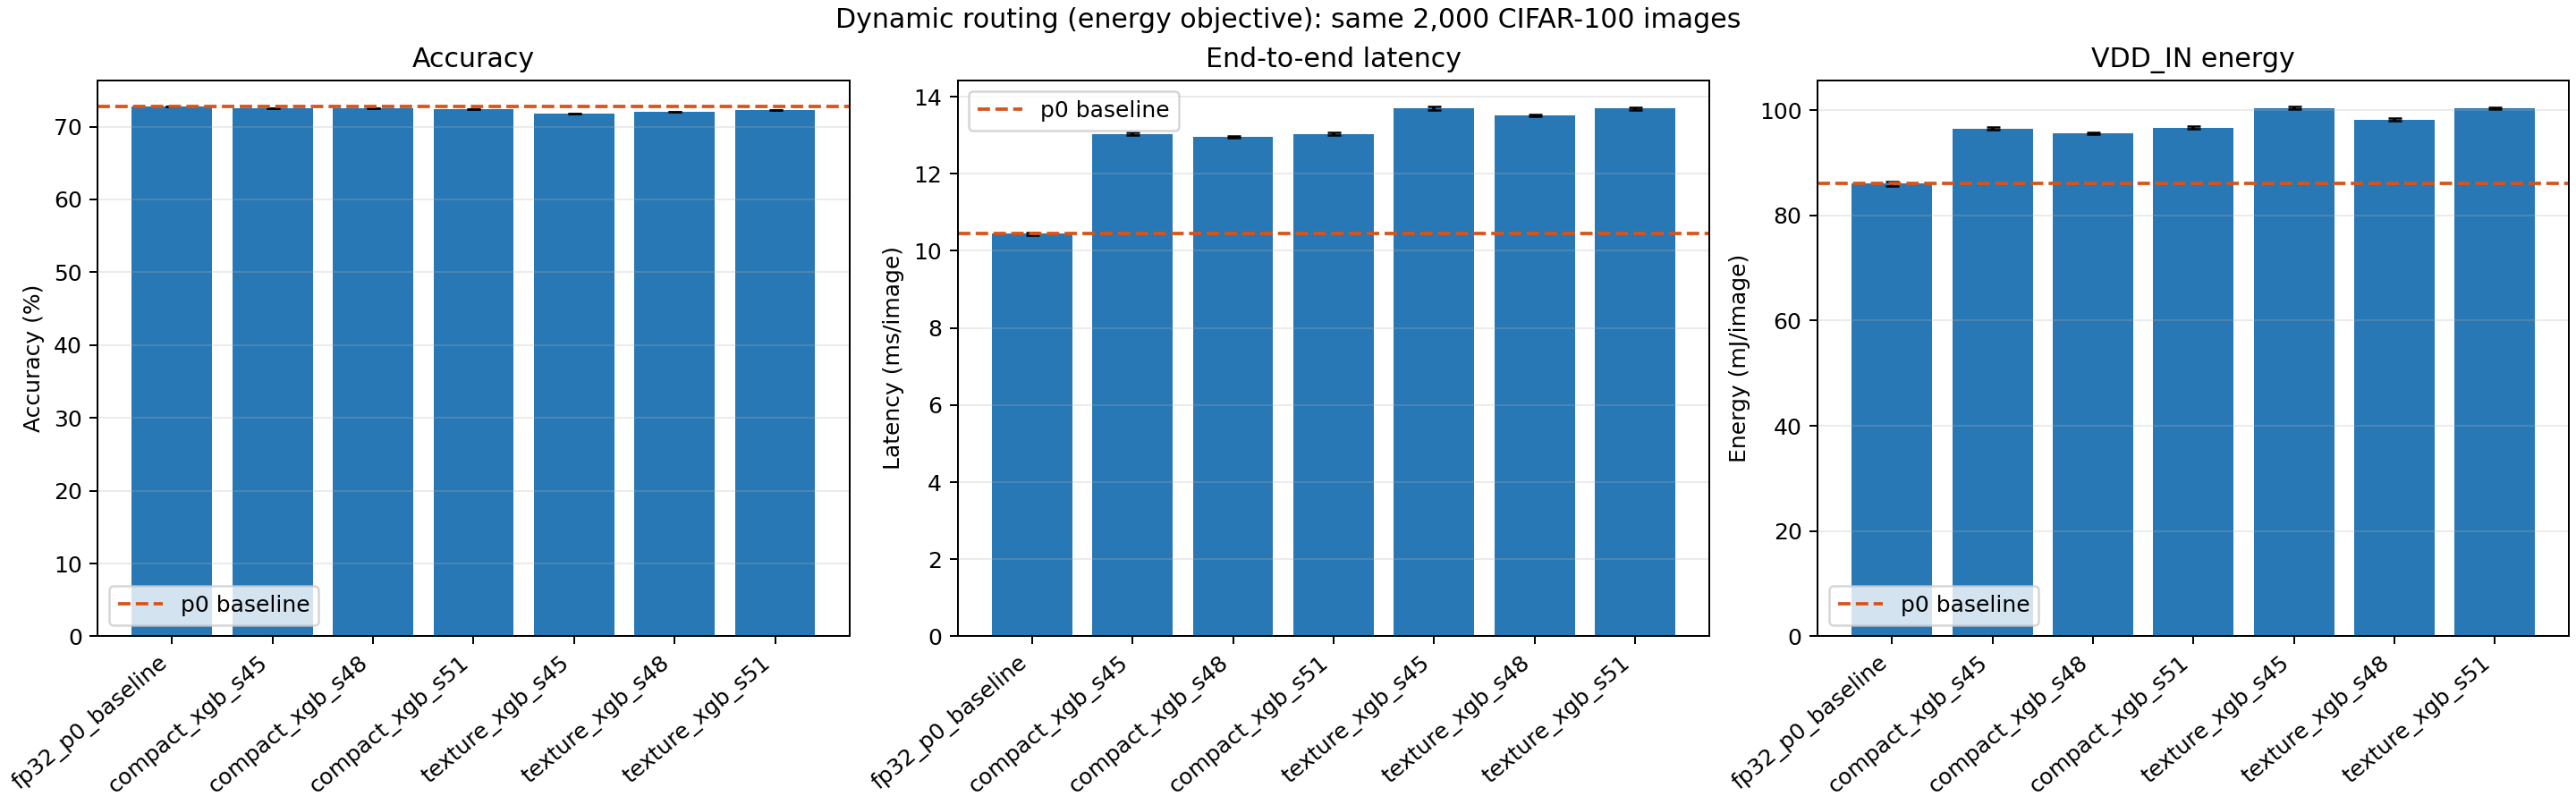
\includegraphics[width=\textwidth]{assets/energy_system_comparison.png}
\caption{End-to-end energy-oriented routing result. The routed systems retain similar accuracy, but router and preprocessing overhead dominate the small savings obtained from mostly selecting mildly pruned models.}
\label{fig:energy-routing}
\end{figure}

This result changes the interpretation of the PC benchmark. A 7--14\% reduction in \emph{candidate} energy is not sufficient evidence of a useful system. When the candidate network itself is already fast, routing must either be extremely cheap or route a substantial fraction of inputs to configurations with much larger cost separation.

\section{Batch-level routing on the Jetson}

Batch routing makes one decision for the complete batch rather than one decision per image. The first version aggregated per-image TinyCNN scores with the 90th percentile. It reduced the amortized router cost but became conservative as batch size increased, sending most batches to p0 or p10. A subsequent percentile sweep with p0/p30/p50/p70 confirmed that a lower per-image overhead alone was not sufficient under the strict accuracy limit.

The current experiment uses p0, p10, p20, and p30. These intermediate candidates were added because the accuracy gap between p0 and p30 was too large for a 0.5-point constraint. Six routers were evaluated: a gradient stump, depth-3 decision tree, logistic regression, depth-2 XGBoost, PyTorch TinyCNN, and FP16 TensorRT TinyCNN. The TinyCNN receives a $4\times4$ grid of $8\times8$ thumbnails sampled from the batch. Batch sizes 32, 64, and 128 and accuracy allowances of 0.5, 1.0, 1.5, and 2.0 percentage points were tested on the same stratified 2,000-image subset. Each complete-system measurement was repeated three times.

Energy and latency were evaluated as separate policies. The energy run used a fixed 624.75 MHz GPU clock; the latency run used 612 MHz. Both measurements include input analysis, routing, transfers, selected-model execution, and synchronization. Energy is obtained by integrating VDD\_IN over the benchmark interval. The direct p0 measurement bypasses the router and is repeated at the same batch size.

The p0 accuracy on this fixed subset is 72.55\%. This does not replace the earlier 73.70\% result, which was measured on the complete 10,000-image test set.

\subsection{Strict 0.5-point allowance}

\begin{table}[H]
\centering
\small
\caption{Best dynamic policies relative to direct p0. Positive savings are improvements; negative values are penalties.}
\begin{tabular}{@{}rlrrrr@{}}
\toprule
Objective & Batch & Router & Accuracy $\Delta$ & Energy saving & Latency saving \\
\midrule
Energy & 32  & Logistic & 0.00\pp  & 2.45\% & $-2.75$\% \\
Energy & 64  & TensorRT TinyCNN & +0.75\pp & 0.07\% & $-2.24$\% \\
Energy & 128 & Logistic & +0.10\pp & 4.90\% & 2.74\% \\
Latency & 32  & Logistic & 0.00\pp & 2.83\% & $-2.17$\% \\
Latency & 64  & TensorRT TinyCNN & +0.75\pp & $-0.57$\% & $-2.68$\% \\
Latency & 128 & Logistic & +0.10\pp & 4.05\% & 1.16\% \\
\bottomrule
\end{tabular}
\label{tab:new-batch-routing}
\end{table}

The apparent positive accuracy differences are possible because pruned and unpruned models make different errors on the same images. They are measured routed-system results, not oracle values.

\begin{table}[H]
\centering
\small
\caption{Static p10 relative to p0 under the same 0.5-point allowance.}
\begin{tabular}{@{}rrrrr@{}}
\toprule
Batch & Accuracy & Accuracy $\Delta$ & Energy saving & Latency saving \\
\midrule
32  & 72.50\% & $-0.05$\pp & 10.13\% & 7.98\% \\
64  & 72.50\% & $-0.05$\pp & 9.30\% & 7.41\% \\
128 & 72.50\% & $-0.05$\pp & 8.80\% & 7.16\% \\
\bottomrule
\end{tabular}
\label{tab:static-p10}
\end{table}

Static p10 is therefore the best deployment choice under the strict limit. The best dynamic policies spend about 5.1 ms per batch at batch 32, 6.0 ms at batch 64, and 11.1 ms at batch 128. TensorRT reduces TinyCNN execution time, but routing quality and the limited p0--p20 cost gap prevent the dynamic policy from recovering this overhead.

\begin{figure}[H]
\centering
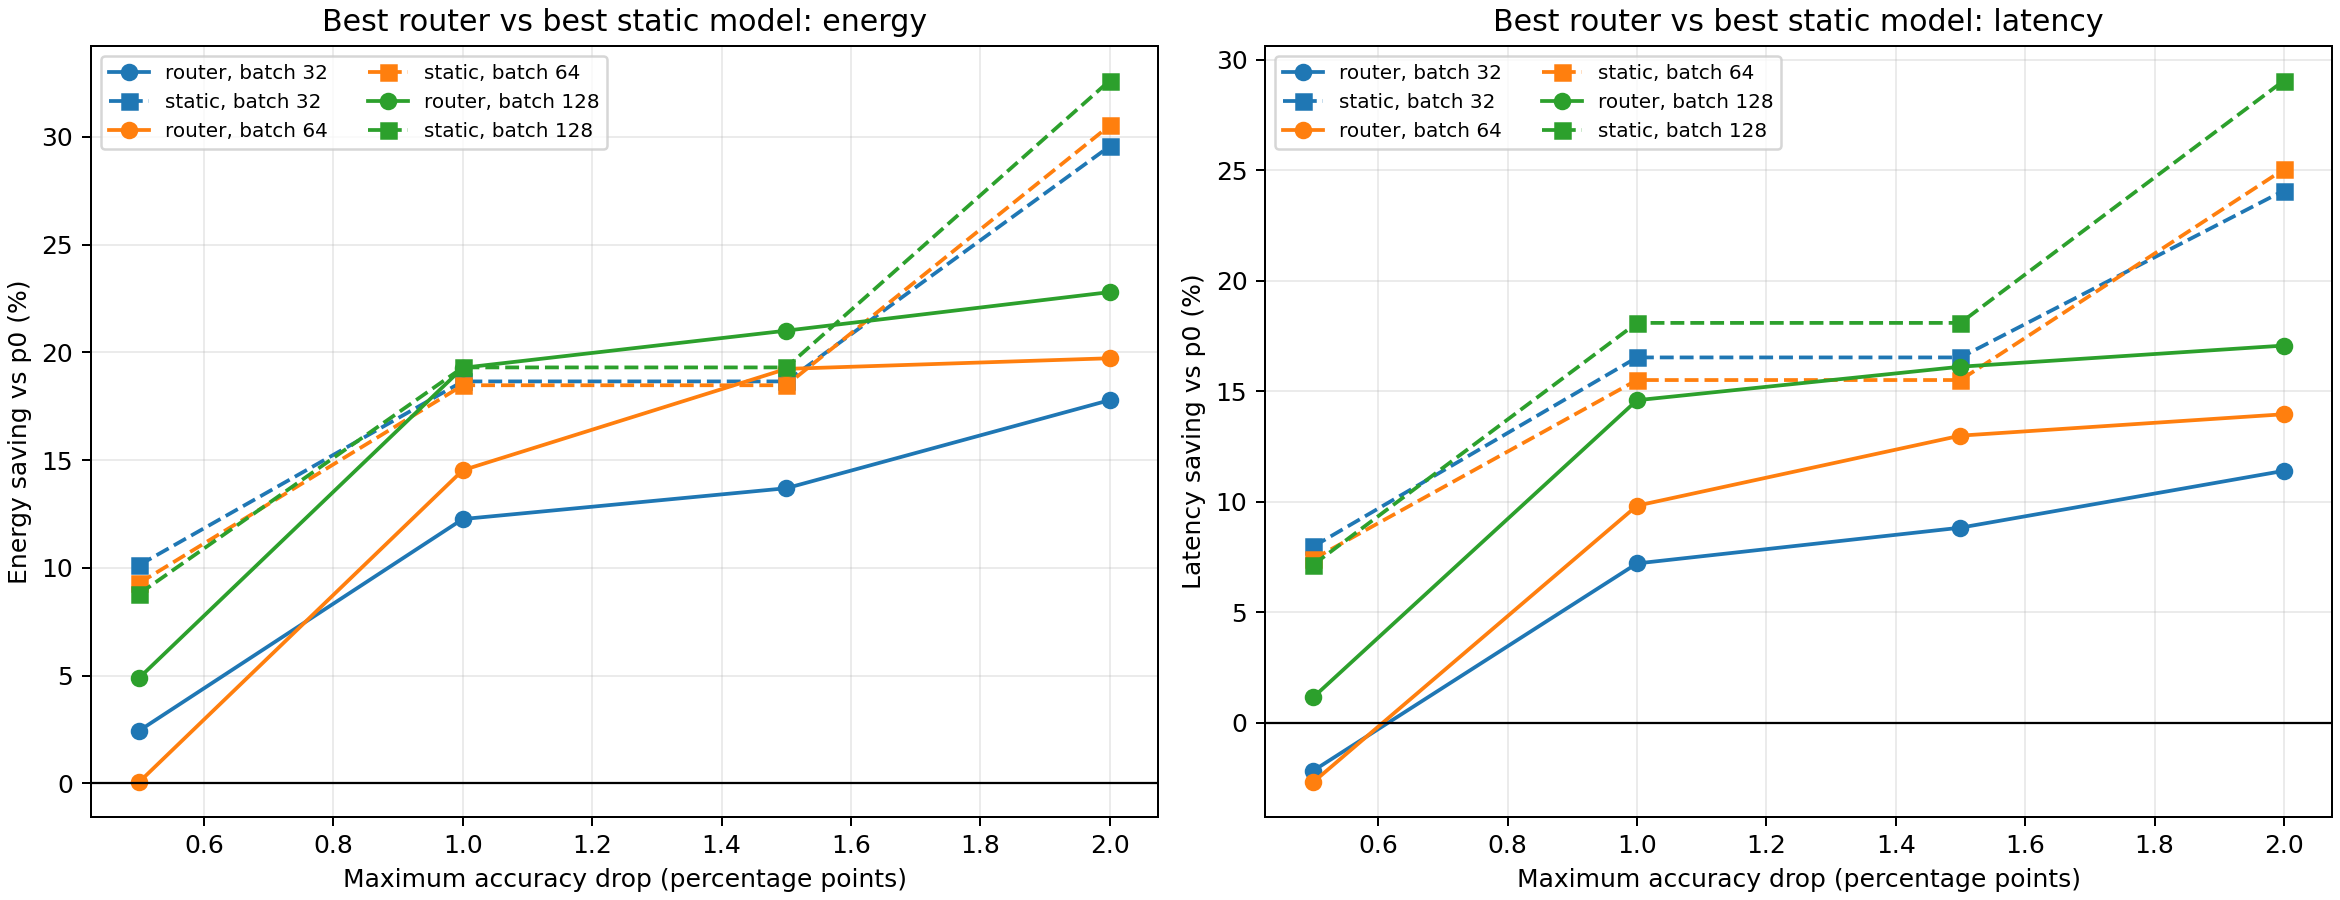
\includegraphics[width=\textwidth]{assets/best_router_vs_static.png}
\caption{Best measured router and best eligible static candidate at each batch size and accuracy allowance. All values are relative to direct p0 execution.}
\label{fig:router-static}
\end{figure}

\subsection{Accuracy--saving trade-off}

At batch 128, the energy policy saves 19.29\%, 21.01\%, and 22.80\% at 1.0, 1.5, and 2.0-point allowances. The latency policy saves 14.59\%, 16.11\%, and 17.07\%. Static models remain better in most cases. The main exception is the energy objective at 1.5 points: the best router saves 19.24\% at batch 64 and 21.01\% at batch 128, compared with 18.48\% and 19.31\% for the best eligible static model. At the 2.0-point allowance, static p30 again dominates, reaching 32.62\% energy and 29.06\% latency savings at batch 128.

\begin{figure}[H]
\centering
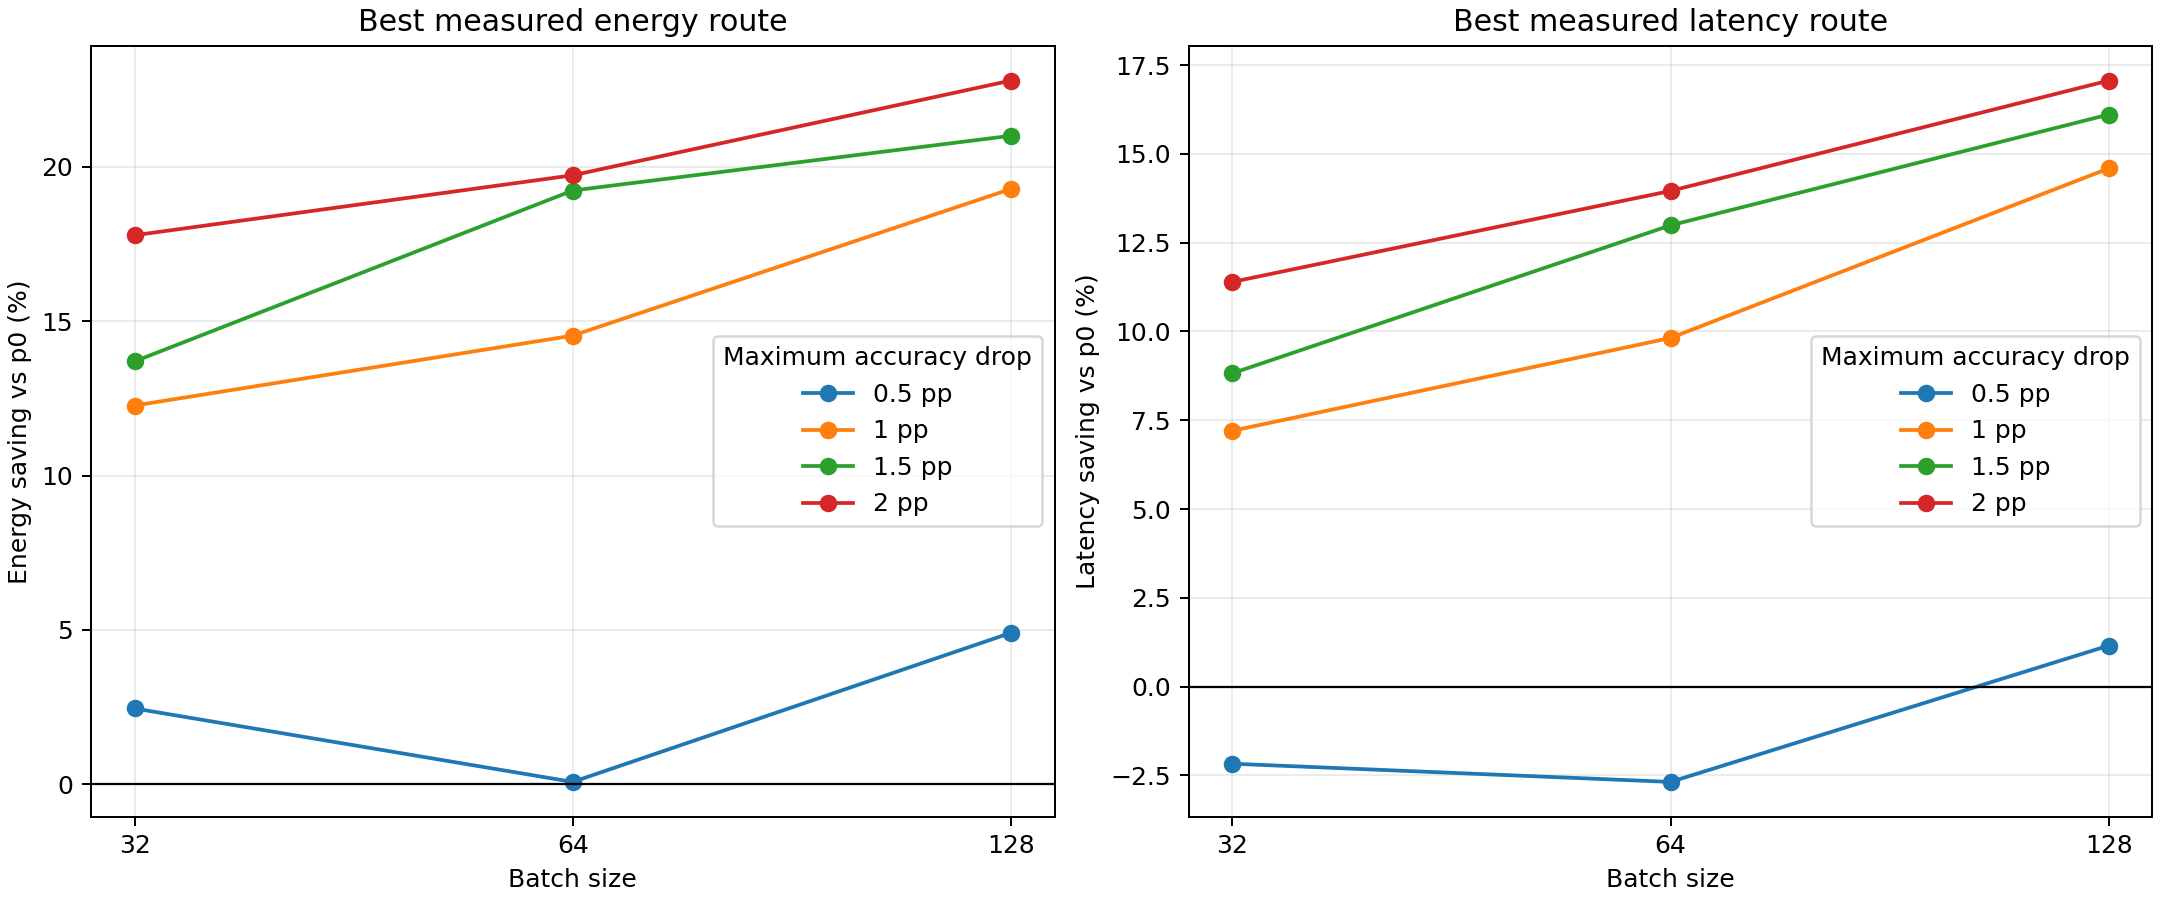
\includegraphics[width=0.94\textwidth]{assets/best_savings_by_accuracy_budget.png}
\caption{Measured saving as the allowed accuracy loss is relaxed. Energy and latency policies are calibrated and reported separately.}
\label{fig:accuracy-saving}
\end{figure}

Under the strict policy, the selected image counts are identical for the best energy and latency routers: 1,008 p0 and 992 p20 images at batch 32; 1,152 p0 and 848 p10 images at batch 64; and 1,280 p0 and 720 p20 images at batch 128. These counts show that the router uses the pruned candidates, but not often enough to outperform static p10.

\begin{figure}[H]
\centering
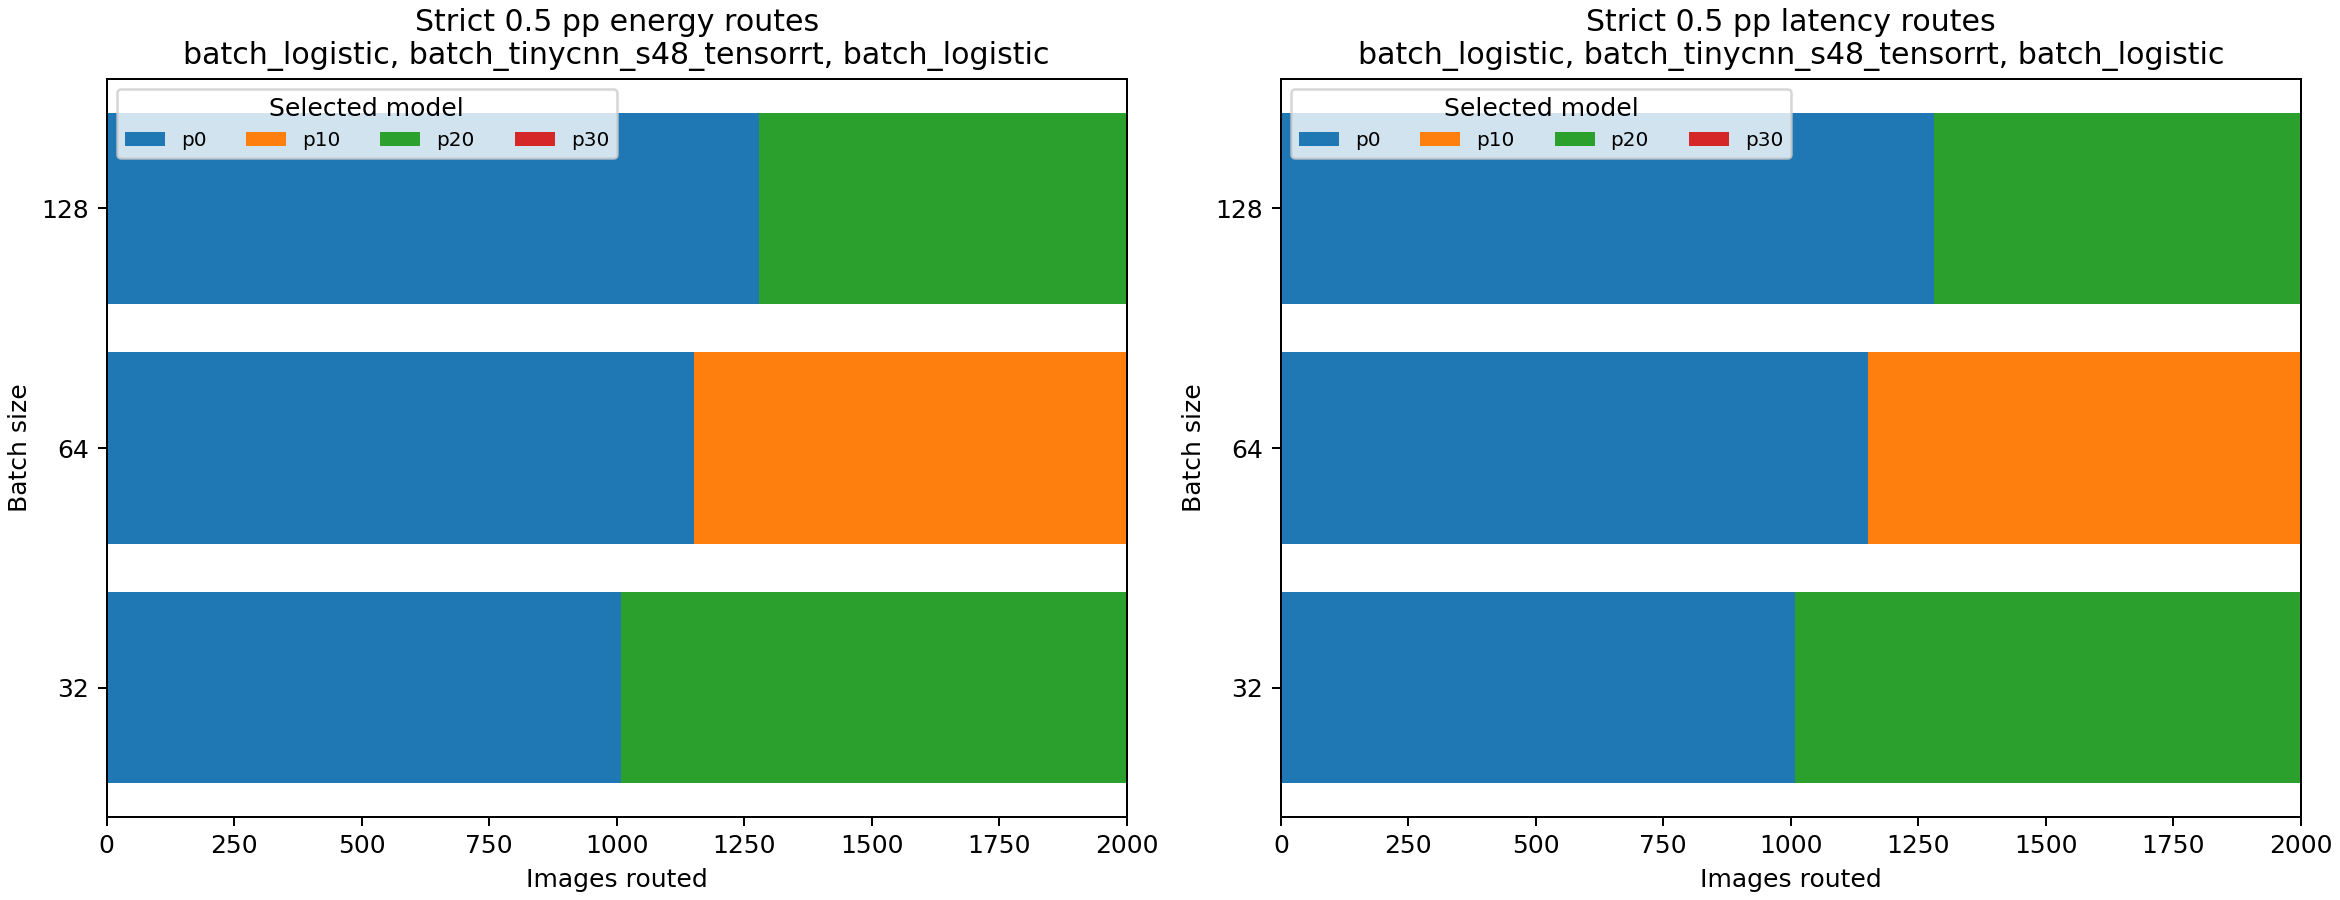
\includegraphics[width=0.88\textwidth]{assets/strict_policy_model_selections.png}
\caption{Model selections for the best strict policy. Counts are reported by image so batch sizes can be compared directly.}
\label{fig:model-selections}
\end{figure}

\section{Findings and limitations}

The measurements support four conclusions. First, the lowest-power hardware mode is not necessarily the lowest-energy mode because a slower execution can keep the module active for longer. Second, pruning level, numerical precision, TensorRT engine profile, and GPU clock must be evaluated together rather than inferred from nominal settings. Third, router overhead must be included in deployment comparisons; candidate-only savings substantially overstated the benefit of the early policies. Fourth, the candidate set matters as much as the router. Closely related ResNet-18 variants have limited cost separation and correlated errors, which leaves little margin for a pre-inference decision.

The results are limited to the ResNet-18 candidate family. ResNet-34 and ResNet-50 have passed structural Torch-Pruning tests, but they have not yet been trained, fine-tuned, exported, and measured under the same CIFAR-100 protocol. The current batch study uses a fixed 2,000-image subset and three system repeats. Router execution is measured end to end, but parts of preprocessing and control flow remain in Python. Finally, the observed trade-offs depend on the chosen accuracy allowance; no single policy is best for all application constraints.

\section{Planned experiments}

\begin{table}[H]
\centering
\small
\caption{Planned work following the current Jetson study.}
\begin{tabularx}{\textwidth}{@{}p{0.23\textwidth}X X@{}}
\toprule
Task & Reason & Expected output \\
\midrule
Fuse the decision path & Remove duplicated preprocessing, transfers, and synchronization & Direct measurement of the minimum practical router overhead \\
Add heterogeneous candidates & Increase error diversity and cost separation using architecture, precision, and pruning & A small Pareto-filtered deployment catalogue \\
Train ResNet-34/50 & Replace the current structural smoke test with a fair accuracy and recovery study & CIFAR-100 accuracy, latency, and energy under equal schedules \\
Add a model-derived baseline & Compare the input-only router with confidence/entropy cascades or early exit & End-to-end comparison of pre-inference and partial-inference decisions \\
Increase repetitions & Quantify run-to-run variation at the most relevant operating points & Confidence intervals for the final deployment comparison \\
\bottomrule
\end{tabularx}
\end{table}

The later optimization problem will treat a candidate as a measured configuration
\[
c=(\text{architecture},\text{pruning},\text{precision},\text{power mode},f_{\mathrm{GPU}},\text{batch size})
\]
and retain only Pareto-efficient points. Energy and latency will remain separate objectives until the individual trade-offs are established. A constrained energy policy can then be written as
\begin{align}
\min_{\pi} \quad & \mathbb{E}[E_{\pi(x)}] \\
\text{s.t.}\quad & A(\pi) \geq A_{p0}-\delta_A, \\
& \mathbb{E}[L_{\pi(x)}] \leq L_{\max}.
\end{align}

\appendix

\section{Detailed routing mechanisms}
\label{app:routing}

\subsection{Handcrafted-feature routers}

The simplest router converts each RGB image into a compact numeric descriptor and feeds it to a classical learner such as XGBoost. The repository implements several levels of descriptor complexity.

The 19-feature basic descriptor contains RGB channel means and standard deviations; grayscale mean, standard deviation, entropy, 10th/90th percentiles and dynamic range; gradient mean/standard deviation and edge density; Laplacian absolute mean and variance; and saturation mean/standard deviation. These features are cheap and interpretable, but they primarily describe image statistics rather than semantic ambiguity.

The 46-feature compact descriptor adds spatial color statistics over four image quadrants and center-versus-border intensity. The 450-feature texture descriptor further adds RGB and grayscale histograms, HOG descriptors, and rotation-invariant local binary patterns. These variants test whether richer non-neural visual structure improves routing enough to justify its extraction cost.

The principal advantage of this family is deployment simplicity: no neural router is necessary and feature importance can be inspected. The main limitation is that a sharp, high-contrast image can still be semantically difficult, while a low-quality image can remain easy for a specific class decision.

\subsection{TinyCNN router}

The TinyCNN uses depthwise-separable convolutions to keep the learned router small. In simplified form:

\begin{lstlisting}
Conv(3 -> 16, 3x3) + BN + ReLU
DepthwiseConv(16) -> PointwiseConv(16 -> 24) + BN + ReLU
DepthwiseConv(24, stride=2) -> PointwiseConv(24 -> 32) + BN + ReLU
DepthwiseConv(32, stride=2) -> PointwiseConv(32 -> 48) + BN + ReLU
AdaptiveAvgPool -> Linear(48 -> output)
\end{lstlisting}

The same architecture is evaluated with 8$\times$8, 16$\times$16, and 32$\times$32 inputs. For scalar routing it produces one difficulty score; for correctness routing the final layer is expanded to one output per candidate model. Compared with handcrafted features, it can learn task-specific semantic cues. Its main risk is that router inference itself becomes a significant fraction of total latency when the selected TensorRT models are very fast.

\subsection{Frozen MobileNet embedding}

The frozen-embedding router uses ImageNet-pretrained MobileNetV3-Small as a feature extractor, freezes its parameters, applies global pooling, and trains an XGBoost model on the resulting embedding. This method produced the largest stable candidate-energy saving in the PC benchmark, but its measured PC overhead was approximately 17 ms per image. It therefore serves as evidence that richer semantic information improves routing quality while also illustrating why the information source must be evaluated together with its computational cost.

\subsection{Scalar, correctness, and advantage targets}

\paragraph{Scalar target.} Candidates are sorted by objective-specific measured cost. For each image, the offline target is the cheapest candidate that predicts correctly; if no candidate is correct, the target falls back to the position of p0. The position is normalized to $[0,1]$ and learned as a regression problem. Calibration then maps the scalar score to a candidate using thresholds and a learned bias.

\paragraph{Correctness target.} The router estimates $P(\text{candidate }m\text{ correct}\mid x)$ for every candidate. The policy combines this estimate with candidate cost through Eq.~\eqref{eq:utility}. This is more expressive than a single scalar because it does not assume that candidate behavior is perfectly ordered by pruning ratio.

\paragraph{Advantage target.} The router estimates whether candidate $m$ is better or worse than p0 on the current image. This is related to the ``benefit of additional computation'' perspective in DynamicDet \cite{dynamicdet}; it focuses on the marginal value of a configuration rather than on generic image difficulty.

\subsection{Why calibration is separated from training}

The 6,000/2,000/2,000 fit/calibration/evaluation split gives different roles to learning, policy selection, and final reporting. Router parameters are learned on the fit set. The calibration set selects the cost penalty or scalar threshold under the accuracy budget. The evaluation set is held out for the reported comparison. This prevents the routing threshold from being tuned directly on the final reported samples.

\subsection{Batch routing}

For batch routing, each image receives a scalar difficulty score. If a batch contains scores $s_1,\ldots,s_B$, the batch decision uses
\begin{equation}
 s_{\mathrm{batch}}=Q_q(s_1,\ldots,s_B),
\end{equation}
where $Q_q$ is a selected percentile. The initial experiment used $q=90\%$ as a conservative rule. The advantage is that neural-router execution can be amortized over the batch and only one TensorRT engine is used. The disadvantage is that high percentiles become increasingly conservative as $B$ grows, because a single difficult input can force the entire batch toward a more expensive model.

\section{Power measurement and hardware controls}
\label{app:power}

The Jetson experiments distinguish nominal configuration from measured consumption. \code{nvpmodel} selects a board-level power/performance profile; GPU frequency is fixed to supported frequencies within the profile. The current manifest contains:

\begin{table}[H]
\centering
\begin{tabular}{@{}lrr@{}}
\toprule
Profile & nvpmodel & Fixed GPU frequency \\
\midrule
7W-306MHz & 1 & 306 MHz \\
7W-408MHz & 1 & 408 MHz \\
15W-306MHz & 0 & 306 MHz \\
15W-408MHz & 0 & 408 MHz \\
15W-510MHz & 0 & 510 MHz \\
15W-612MHz & 0 & 612 MHz \\
15W-624.75MHz & 0 & 624.75 MHz \\
\bottomrule
\end{tabular}
\end{table}

Power is sampled with \code{tegrastats}. The main reporting rail is \code{VDD\_IN}, representing total module input power; \code{VDD\_CPU\_GPU\_CV} is also recorded as a combined compute-domain rail. Energy is integrated over the measured interval and normalized by image count:
\begin{equation}
 E_{\mathrm{image}} = \frac{1}{N}\int_{t_0}^{t_1}P_{\mathrm{VDD\_IN}}(t)\,dt.
\end{equation}

This is preferred to multiplying a nominal 7 W or 15 W label by runtime because actual consumption depends on workload, clocks, utilization, and batch size.

\section{Structural ResNet-34/50 pruning results}
\label{app:pruning}

\begin{longtable}{@{}rr|rr|rr@{}}
\caption{Torch-Pruning structural validation. All configurations passed a forward pass with 100 output classes.}\label{tab:structural-pruning}\\
\toprule
\multicolumn{2}{c|}{Requested} & \multicolumn{2}{c|}{ResNet-34 reduction} & \multicolumn{2}{c}{ResNet-50 reduction} \\
Ratio & & MACs & Params & MACs & Params \\
\midrule
\endfirsthead
\toprule
Ratio & & R34 MACs & R34 Params & R50 MACs & R50 Params \\
\midrule
\endhead
10\% && 22.59\% & 21.78\% & 21.84\% & 20.89\% \\
20\% && 40.14\% & 37.80\% & 38.96\% & 37.17\% \\
30\% && 53.81\% & 52.76\% & 52.99\% & 52.15\% \\
40\% && 67.10\% & 65.00\% & 66.05\% & 64.60\% \\
50\% && 74.12\% & 74.91\% & 74.08\% & 74.72\% \\
60\% && 84.91\% & 85.15\% & 84.56\% & 84.61\% \\
70\% && 92.06\% & 91.60\% & 91.62\% & 91.26\% \\
80\% && 96.55\% & 96.46\% & 96.32\% & 96.21\% \\
90\% && 77.06\% & 98.03\% & 86.86\% & 98.47\% \\
\bottomrule
\end{longtable}

The 90\% row is intentionally retained because it demonstrates why requested channel ratio, parameter count, MAC count, and actual deployment cost should all be reported separately.

\section{Literature map used to define the thesis direction}
\label{app:literature}

The literature review covered 21 papers. The table below records the role each paper played in defining the current thesis rather than reproducing a full paper-by-paper review.

\begin{longtable}{@{}p{0.26\textwidth}p{0.18\textwidth}p{0.49\textwidth}@{}}
\caption{Literature map.}\label{tab:literature-map}\\
\toprule
Paper & Topic & Relevance to the thesis \\
\midrule
\endfirsthead
\toprule
Paper & Topic & Relevance to the thesis \\
\midrule
\endhead
Dynamic Neural Networks: A Survey \cite{han2021dynamic} & Dynamic inference taxonomy & Positions model routing, dynamic depth, width, spatial and temporal adaptation under one framework. \\
Conditional Computation \cite{scardapane2024conditional} & Conditional sparsity / routing & Provides a common view of gates, hard/soft routing, expert selection, and routing overhead. \\
Adaptive Inference through Early-Exit Networks \cite{laskaridis2021} & Early-exit design & Defines exit placement, training, confidence policies, calibration, and deployment considerations. \\
BranchyNet \cite{branchynet} & Early exit & Canonical confidence-based intermediate exits; baseline for dynamic depth. \\
MSDNet \cite{msdnet} & Early exit / multi-scale features & Architecture designed to support strong intermediate predictions. \\
SkipNet \cite{skipnet} & Block skipping & Learns per-input residual-block execution; shows fine-grained conditional computation. \\
Once-for-All \cite{ofa} & Elastic subnetworks & Demonstrates one trained supernetwork specialized to hardware constraints. \\
DynamicViT \cite{dynamicvit} & Token pruning & Dynamic token sparsification; example of input-adaptive computation inside a transformer. \\
PTEENet \cite{pteenet} & Post-trained early exit & Relevant to adding exits without redesigning the full backbone. \\
DyCE \cite{dyce} & Configurable early exit & Connects early exit with compression and real-time scaling. \\
Predictive Exit \cite{predictiveexit} & Exit prediction + energy & Predicts future exit behavior and considers hardware/DVFS implications. \\
PolyThrottle \cite{polythrottle} & Hardware-aware optimization & Uses constrained optimization for energy-efficient edge inference under latency objectives. \\
E4 \cite{e4} & Early exit + DVFS & Directly motivates combining algorithmic decisions with hardware power/frequency control. \\
Hardware-Algorithm Co-Optimization \cite{zniber2026} & Joint accelerator/EE design & Motivates co-optimizing exits, quantization, mapping, memory traffic, latency, and energy. \\
Comparative Study of CNN Optimization Methods \cite{fernandez2026} & Unified comparison & Supports comparing pruning, quantization, early exit, and combinations under one deployment protocol. \\
Adaptive Neural Networks for Efficient Inference \cite{bolukbasi2017} & Sequential cascade & Small-to-large escalation based on uncertainty; useful contrast with pre-inference routing. \\
IF-CNN \cite{shu2018ifcnn} & Pre-inference model selection & One of the closest historical examples of image-aware selection among CNNs. \\
PERTINENCE \cite{shende2026pertinence} & Input-based model routing & Closest conceptual neighbor: offline candidate behavior and input-based dispatch to an efficient model. \\
CARN \cite{gaire2025carn} & Complexity-aware routing & Routes among computation levels using learned/shared representations and complexity-aware objectives. \\
DynamicDet \cite{dynamicdet} & Benefit-based difficulty & Defines difficulty through the improvement obtained from extra computation, supporting a marginal-benefit view. \\
DualRes \cite{dualres2026} & Dynamic resolution & Production-oriented pre-inference routing; emphasizes deployment overhead and ONNX/runtime behavior. \\
\bottomrule
\end{longtable}

\section{Repository reproducibility notes}
\label{app:repro}

The repository intentionally separates PC and Jetson dependencies. The following commands summarize the main reproducible stages.

\subsection{PC router benchmark}
\begin{lstlisting}
python run_refined_routers.py \
  --data-dir <cifar100-data> \
  --output-dir artifacts/refined_energy \
  --objective energy

python run_refined_routers.py \
  --data-dir <cifar100-data> \
  --output-dir artifacts/refined_latency \
  --objective latency
\end{lstlisting}

\subsection{Jetson power sweep}
\begin{lstlisting}
sudo nvpmodel -q --verbose

python scripts/run_power_sweep.py \
  --experiment-name hardware_characterization \
  --model-pattern '^distilled_resnet18$' \
  --precisions fp16 --batch-sizes 1,32
\end{lstlisting}

\subsection{Jetson dynamic routing}
\begin{lstlisting}
python scripts/benchmark_dynamic_routing.py \
  --manifest manifests/dynamic_routers.energy.json \
  --trt-engine-dir outputs/tensorrt/engines/fp32 \
  --output-dir results/dynamic_routing_energy \
  --batch-sizes 8,16,32 \
  --difficulty-percentile 90
\end{lstlisting}

The most recent p0/p30/p50/p70 engines were rebuilt directly on the current Jetson with profiles up to batch 128. The completed energy sweep and its raw tables should be preserved separately from the earlier batch-32/90th-percentile report because they use a different candidate set and accuracy budget. The corresponding latency sweep should be completed before producing publication-quality combined tables.

For publication-quality experiments, warm-up and measurement protocols should be frozen, power mode and GPU clock should be recorded with every run, and raw run-level CSVs should be retained even if only concise summaries are committed to the repository.

\clearpage
\begin{thebibliography}{99}
\small
\bibitem{han2021dynamic} Y. Han et al., ``Dynamic Neural Networks: A Survey,'' arXiv:2102.04906, 2021.
\bibitem{scardapane2024conditional} S. Scardapane et al., ``Conditional Computation in Neural Networks: Principles and Research Trends,'' arXiv:2403.07965, 2024.
\bibitem{laskaridis2021} S. Laskaridis, A. Kouris, and N. D. Lane, ``Adaptive Inference through Early-Exit Networks: Design, Challenges and Directions,'' EMDL, 2021.
\bibitem{branchynet} S. Teerapittayanon, B. McDanel, and H. T. Kung, ``BranchyNet: Fast Inference via Early Exiting from Deep Neural Networks,'' ICPR, 2016; arXiv:1709.01686.
\bibitem{msdnet} G. Huang et al., ``Multi-Scale Dense Networks for Resource Efficient Image Classification,'' ICLR, 2018; arXiv:1703.09844.
\bibitem{skipnet} X. Wang et al., ``SkipNet: Learning Dynamic Routing in Convolutional Networks,'' ECCV, 2018.
\bibitem{ofa} H. Cai et al., ``Once-for-All: Train One Network and Specialize It for Efficient Deployment,'' ICLR, 2020.
\bibitem{dynamicvit} Y. Rao et al., ``DynamicViT: Efficient Vision Transformers with Dynamic Token Sparsification,'' NeurIPS, 2021.
\bibitem{pteenet} A. Lahiany and Y. Aperstein, ``PTEENet: Post-Trained Early-Exit Neural Networks Augmentation for Inference Cost Optimization,'' arXiv:2501.02508, 2025.
\bibitem{dyce} Q. Wang et al., ``DyCE: Dynamically Configurable Exiting for Deep Learning Compression and Real-Time Scaling,'' arXiv:2403.01695, version 2025.
\bibitem{predictiveexit} X. Li et al., ``Predictive Exit: Prediction of Fine-Grained Early Exits for Computation- and Energy-Efficient Inference,'' AAAI, 2023.
\bibitem{polythrottle} M. Yan and H. Wang, ``PolyThrottle: Energy-Efficient Neural Network Inference on Edge Devices,'' arXiv:2310.19991, 2024.
\bibitem{e4} Z. Zhang et al., ``E4: Energy-Efficient DNN Inference for Edge Video Analytics via Early-Exit and DVFS,'' arXiv:2503.04865, 2025.
\bibitem{zniber2026} A. Zniber et al., ``Hardware-Algorithm Co-Optimization of Early-Exit Neural Networks for Multi-Core Edge Accelerators,'' arXiv:2512.04705, 2026 version.
\bibitem{fernandez2026} N. Fernandez et al., ``A Comparative Study of CNN Optimization Methods for Edge AI: Exploring the Role of Early Exits,'' arXiv:2604.14789, 2026.
\bibitem{bolukbasi2017} T. Bolukbasi, J. Wang, O. Dekel, and V. Saligrama, ``Adaptive Neural Networks for Efficient Inference,'' ICML, PMLR 70, 2017.
\bibitem{shu2018ifcnn} G. Shu, W. Liu, X. Zheng, and J. Li, ``IF-CNN: Image-Aware Inference Framework for CNN with the Collaboration of Mobile Devices and Cloud,'' IEEE Access, vol. 6, 2018.
\bibitem{shende2026pertinence} O. Shende, G. Ananthanarayanan, and M. Traiola, ``PERTINENCE: Input-Based Opportunistic Neural Network Dynamic Execution,'' IEEE Access, 2026.
\bibitem{gaire2025carn} R. Gaire and A. Roohi, ``CARN: Complexity-Aware Routing Network for Efficient and Adaptive Inference,'' CVPR Workshop, 2025.
\bibitem{dynamicdet} Z. Lin, Y. Wang, J. Zhang, and X. Chu, ``DynamicDet: A Unified Dynamic Architecture for Object Detection,'' CVPR, 2023.
\bibitem{dualres2026} J. El Hassani and T. Verelst, ``DualRes: Production-Ready Dynamic Object Detection,'' WACV, 2026.
\end{thebibliography}

\end{document}
